% !TeX encoding = UTF-8
% !TeX spellcheck = de_DE

\RequirePackage[l2tabu, orthodox]{nag}

\documentclass[utf8,biblatex]{lni}
\bibliography{bibliographie.bib}

\usepackage{booktabs}

\usepackage[math]{blindtext}
\usepackage{mwe}
\usepackage[toc,page]{appendix}
\usepackage{tikz}
\usepackage{tkz-kiviat} 
\usetikzlibrary{arrows}
\usepackage{pgfplots}
\usepackage{etoolbox}

\renewcommand{\appendixtocname}{Anhang}
\renewcommand{\appendixpagename}{Anhang}

\makeatletter
\patchcmd{\tkz@KiviatGrad}{\pgfmathresult}{\pgfmathresult-1}
         {\typeout{*** SUCCESS ***}}
         {\ERRORpatchfailed}
\makeatother 


\usepackage{longtable}

\iffalse
\AtEveryBibitem{%
  \ifentrytype{article}{%
  }{%
    \clearfield{doi}%
    \clearfield{issn}%
    \clearfield{url}%
    \clearfield{urldate}%
  }%
  \ifentrytype{inproceedings}{%
  }{%
    \clearfield{doi}%
    \clearfield{issn}%
    \clearfield{url}%
    \clearfield{urldate}%
  }%
}
\fi

\begin{document}

\title[Untersuchung von Web-Usability Prinzipien und Evaluation zweier Webshops]{Untersuchung von Web-Usability Prinzipien und Evaluation zweier Webshops}

\author[Alicia Dietrich \and Nick Dürr \and Jan Perthel]
{Alicia Dietrich\footnote{DHBW Stuttgart Campus Horb, Informatik, Florianstr. 15, 72160 Horb am Neckar, Deutschland, \email{i20005@hb.dhbw-stuttgart.de}} \and
 Nick D\"urr\footnote{DHBW Stuttgart Campus Horb, Informatik, Florianstr. 15, 72160 Horb am Neckar, Deutschland, \email{i20008@hb.dhbw-stuttgart.de}} \and
 Jan Perthel\footnote{DHBW Stuttgart Campus Horb, Informatik, Florianstr. 15, 72160 Horb am Neckar, Deutschland, \email{i20027@hb.dhbw-stuttgart.de}}}

\startpage{1}
\editor{DHBW Stuttgart Campus Horb}
\booktitle{Advanced Software Engineering}
\maketitle



\begin{abstract}
Aufgrund der stetig steigenden Anzahl von Webshops gewinnt Web-Usability immer mehr an Bedeutung. Die vorliegende Seminararbeit beschäftigt sich aus diesem Grund mit der Betrachtung von Prinzipien der Web-Usability nach Nielsen und nach DIN EN ISO 9241-151. Diese Ansätze werden anschließend gegenübergestellt. Um die Einhaltung der Prinzipien sicherzustellen, existieren unterschiedliche Vorgehensweisen. Im Rahmen der Arbeit werden die Usability Inspection, der Usability Engineering Lifecycle und die Menschzentrierte Gestaltung vorgestellt und miteinander verglichen. Danach wird die Usability Inspection am Beispiel von zwei verschiedenen Webshops praktisch umgesetzt. Schlussendlich wird die Anwendbarkeit dieser Vorgehensweise im Bezug auf die Webshops verglichen und evaluiert.
\end{abstract}



\begin{keywords}
Web-Usability, E-Commerce, Heuristiken, Usability Engineering, Usability Inspection
\end{keywords}



\section{Einleitung}


\subsection{Motivation}
In der heutigen Informationsgesellschaft stellt das Internet für viele Unternehmen einen der wichtigsten Verkaufskanäle dar. Mithilfe von Webshops können Unternehmen einfach Produkte oder Dienstleistungen bewerben, an Kunden verkaufen und eine breite Menschenmenge erreichen. Maßgeblich für den Erfolg dieser Verkaufsstrategie ist die Anzahl der Kunden im Verhältnis zur Anzahl der Interessenten. Dieses Verhältnis hängt neben der Beliebtheit der Produkte und des Unternehmens davon ab, wie der Webshop gestaltet ist. Ein ansprechend gestalteter Webshop zieht deutlich mehr Interessenten an. Wichtig ist dabei letztlich nicht nur das Aussehen, sondern auch die Bedienbarkeit (Usability) der Oberfläche. In einer Umfrage von Statista zum Besuch von Online-Fashion-Shops gaben 44 Prozent der Nutzer an, dass Usability ein Kaufs entscheidender Faktor ist. Weitere 41 Prozent gaben sogar an, dass Usability wesentlich ist für die Entscheidung den Webshop zu besuchen oder nicht

In einer Umfrage von Statista zum Besuch von Online-Fashion-Shops gaben 44 Prozent der Nutzer an, dass Usability ein Kaufs entscheidender Faktor ist. Weitere 41 Prozent gaben sogar an, dass Usability wesentlich ist für die Entscheidung den Webshop zu besuchen oder nicht. Lediglich 15 Prozent gaben an Usability sei nicht relevant.\cite{Statista.2022} Beide Faktoren, Design und Usability, sind somit wichtig, um sich gegenüber der breiten Menge an Webshops abzuheben und den Interessenten zu einem erfolgreichen Abschluss des Kaufes oder gar zum Besuch des Webshops zu überzeugen. Doch welche Faktoren beinhalten eine \glqq gute\grqq  Usability und wie kann diese am eigenen Webshop überprüft werden? Diese Frage soll unter anderem im Rahmen der Arbeit geklärt werden.


\subsection{Zielsetzung}
Diese Arbeit soll die Frage klären, welche Usability Heuristiken es gibt und wie diese praktisch umgesetzt werden können. Diese Fragen werden beispielhaft an einem Webshop beantwortet.

Als Ergebnis dieser Arbeit wird ein Katalog an Heuristiken erarbeitet. Dabei werden verschiedene Heuristiken aus der Literatur gegenübergestellt und analysiert welche Heuristiken besonders relevant für das Web sind. 

Daraufhin wird beschrieben, wie die Heuristiken in diesem Katalog während der Entwicklung einer Webseite praktisch umgesetzt werden können. Dabei wird vor allem auf den Usability Engineering Lifecycle, Usability Inspections und die menschenzentrierte Gestaltung eingegangen. Auch werden konkrete Methoden und Hilfsmittel zur Umsetzung des Lifecycles betrachtet.

Schlussendlich wird dieses Vorgehen an zwei verschiedenen Webshops beispielhaft aufgezeigt. Dabei wird überprüft, wie gut das Vorgehen und die Heuristiken auf die verschiedene Arten von Webshops anwendbar sind. 



\section{Grundlagen der Web-Usability} \label{chp:basics}


\subsection{Was ist Web-Usability?}
Um den Begriff der Web-Usability einzuführen, ist es notwendig den Begriff Usability zu betrachten. Usability wird von \cite[]{JakobNielsen.2022} wie folgt definiert: Usability beschreibt ein Attribut, das sich darauf bezieht, wie "leicht" oder einfach etwas zu verwenden ist. Es bezieht sich also darauf, wie schnell ein Nutzer lernen kann eine Software zu verwenden, wie effizient die Nutzung dieser ist und wie gut es im Gedächtnis bleibt. Außerdem wird betrachtet, wie fehleranfällig sie ist und wie viele Nutzer sie gerne verwenden.\cite[]{JakobNielsen.2022}

Bei der Web-Usability steht die Funktion bzw. die Funktionalität der Website im Fokus. Es wird definiert, welchem Zweck die Website erfüllen soll. Die Web-Usability sorgt dafür, dass ein Benutzer eine Website optimal bedienen kann und zudem noch ansprechend und sinnvoll gestaltet ist. Eine Website soll für den Benutzer bezüglich der Bedienung und der Funktionalität möglichst attraktiv sein. 

Nach \cite[]{DINDeutschesInstitutfurNormunge.V..g} wird Usability (zu Deutsch: Gebrauchstauglichkeit) wie folgt definiert: \glqq Ausmaß, in dem ein System, ein Produkt oder eine Dienstleistung durch bestimmte Benutzer in einem
bestimmten Nutzungskontext genutzt werden kann, um bestimmte Ziele effektiv, effizient und
zufriedenstellend zu erreichen\grqq.

Um die Usability einer Website einzuhalten, wurden nach ISO und Nielsen verschiedene Prinzipien definiert, die erfüllt werden müssen, um ein hohes Maß an Usability zu erreichen. Diese Prinzipien werden im Folgenden definiert.


\subsection{Heuristiken der Web-Usability nach Nielsen}\label{chp:heuristics}
Nielsen definiert in \cite{Nielsen.UE} verschiedene Prinzipien, nach denen eine Website oder Weboberfläche gestaltet werden sollte.


\subsubsection{Ästhetisches und minimalistisches Design}
Das erste Prinzip welches Nielsen beschreibt, sagt aus, dass eine Oberfläche möglichst einfach und simpel gehalten werden sollte. Jedes zusätzliche Feature muss vom Nutzer erlernt werden und jedes weitere Feature hat die Möglichkeit missverstanden zu werden. Die Oberfläche sollte dabei möglichst dem natürlichen Verhalten des Nutzer beim Lösen einer Aufgabe entsprechen. Das bedeutet es wäre ideal, wenn zu jedem Zeitpunkt die für den Nutzer benötigten Informationen am passenden Ort angezeigt werden und die Folge der Aktionen und Objekte der Abfolge des Nutzer entspricht. \\
Informationen die zusammen verwendet werden, sollten auch nah beieinander platziert werden. Durch graphische Elemente lassen sich Informationen gruppieren bzw. voneinander trennen. Hierfür können z.B. Linien oder farbliche Abhebungen verwendet werden.\\
Beim Design einer Oberfläche sollte auch der natürliche Lesefluss des Nutzers beachtet werden. Informationen, die weiter oben und links platziert werden, bekommen am meisten und meistens als erstes die Aufmerksamkeit des Nutzers.\\
Für das Design einer Website werden drei wichtige Punkte festgelegt:
\begin{itemize}
  \item Don ‘t over do it: Ein Website sollte nicht aus vielen kontrastreichen und sättigungsreichen Farben bestehen, sondern lieber aus schlichten Farben und einer geringeren Anzahl. Es sollten insgesamt fünf bis sieben verschiedene Farben verwendet werden. Durch eine geringere Anzahl an Farben kann der Nutzer sich besser erinnern.
  \item Die Oberfläche sollte auch ohne Farbe genutzt werden können. Dies ist vor allem für farbenblinde Menschen wichtig. Jede Farbinformation sollte zusätzlich durch Icons symbolisiert werden, sodass eine Oberfläche auch ohne Farben interpretiert werden kann.
  \item Als letzten Punkt sollte beachtet werden, dass eine Farbe nicht zur Informationsbereitstellung genutzt werden sollte, sondern lediglich, um Informationen zu kategorisieren, zu differenzieren und um zu highlighten
\end{itemize}

Das Design der Oberfläche soll nach dem Motto \glqq weniger ist mehr \grqq erstellt werden. Es sollte differenziert werden, welche Informationen wirklich essenziell notwendig sind und welche eventuell in zusätzliche Szenen, wie Hilfsdialoge usw., ausgelagert werden können. Am besten wäre es alle wichtige Informationen innerhalb eines Single Screens darzustellen und bei Bedarf weiterer Informationen weitere Elemente zur Verfügung zu stellen. Das Prinzip von weniger ist mehr gilt nicht nur für das Design der Oberfläche, sondern auch für die Funktionen und Mechanismen, die eine Website zur Verfügung stellt. Dem Nutzer sollen nicht unnötig viele Optionen angeboten werden, dies führt zu Fehlern und zur Verwirrung. Außerdem bedeutet jedes (unnötige) Feature, dass zu einer Software hinzugefügt wird, eine weitere Sache die der Nutzer lernen muss. Dadurch wird die Komplexität einer Software unnötig \glqq aufgebläht \grqq. 


\subsubsection{Übereinstimmung von System und realer Welt}
In diesem Prinzip wird auf Terminologie der Anwendung eingegangen. Die Terminologie der Nutzeroberfläche soll der Sprache des Nutzer entsprechen. Dialoge sollten, wenn möglich, in der nativen Sprache des Nutzer formuliert sein, damit der Nutzer sie gut verstehen kann. Wie beim Design sollen zur Symbolisierung der Nachricht zusätzlich Icons verwendet werden. Innerhalb der Wortwahl sollte darauf geachtet werden, mehrdeutige Wörter möglichst zu vermeiden, um Missverständnisse des Nutzers zu verhindern. Eine Oberfläche sollte trotzdem nicht nur auf ein paar häufig verwendete Wörter beschränkt sein, hat die Community ihre eigene Fachterminologie, so sollten lieber diese verwendet werden. Alle Interaktionen die den Nutzer beinhalten, sollten aus Sicht des Nutzer formuliert sein (z.B. \glqq Sie haben 100 Stück von xyz erworben.\grqq).\\
Insgesamt führt eine besser Terminologie der Oberfläche zu einem besseren Verständnis beim Nutzer und es fällt ihm einfacher die Oberfläche zu Bedienen. Dies steigert die Effizienz im Umgang mit der Anwendung. Um dies weiter zu unterstützen, sollte ein Nutzer für Begriffe Aliase definieren können, die vom System definierte Begriffe ersetzt. Ein System sollte außerdem mitlernen können und sich z.B. Falscheingaben des Nutzers merken und trotzdem passende Ergebnisse zum eigentlich gemeinten Befehl anzeigen.


\subsubsection{Erkennen vor Erinnern}
In diesem Prinzip geht es um die Unterstützung des Systems gegenüber dem Nutzer. Computer können sich, im Gegensatz zu uns Menschen, sehr genau an Dinge erinnern, während wir Menschen eher gut darin sind Dinge wiederzuerkennen. Deshalb sollten Menüs eingeführt werden, die dem Nutzer helfen sich innerhalb einer komplexen Anwendung zurechtzufinden. \\
Die Anwendung sollte den Nutzer darin unterstützen, sich an verschiedene Informationen zu erinnern. Dies kann umgesetzt werden, indem z.B. beim Bearbeiten eines Eintrags alle Felder mit den aktuell bestehenden Informationen zum Eintrag vorausgefüllt werden. Der Nutzer muss sich so nicht an alle Informationen zurückerinnern. Um Fehler zu vermeiden, sollte die Software bei der Eingabe von Informationen immer auf die gewünschte Form hinweisen, um später auftretende Fehler zu verhindern.\\
Ein System sollte außerdem auf einer kleinen Menge an Regeln basieren, die der Nutzer lernen muss. Je mehr Regeln der Nutzer lernen muss, desto schwieriger ist es für ihn, sich an alle zu erinnern. Es muss ein gutes Mittelmaß gefunden werden, wie viele Regeln ein System besitzt, denn ganz ohne Regeln kommt ein System auch nicht aus. Dann ist es schwierig für den Nutzer das Verhalten verschiedener Elemente zu verstehen bzw. vorherzusagen. 


\subsubsection{Konsistenz und Standardisierung}
Konsistenz innerhalb der Usability bedeutet, dass gleich ausgeführten Aktionen zu identischen Ergebnissen führen sollten. Die Software soll immer das gleiche Verhalten und die gleiche Reaktion auf identisch ausgeführte Aktionen zeigen. Durch Konsistenz erhält der Nutzer mehr Sicherheit im Umgang mit der Software und neue Dinge können schneller erlernt werden.\\
Zudem sollten gleiche Informationen immer an gleichen Stellen zu finden sein und mit gleicher Formatierung. Informationen die sich aufeinander beziehen sollten auch in der gleichen Reihenfolge vorzufinden sein. Als Beispiel sei eine Tabelle gegeben mit Daten aus dem Jahr und Vorjahr. Die Zusatzinformation, die zu dieser Tabelle formuliert wird, soll sich dann ebenfalls in der Reihenfolge Vorjahr und Jahr befinden und nicht umgekehrt. \\
Konsistenz sollte auch bei den Aufgaben eines Systems beachtet werden.


\subsubsection{Sichtbarkeit des Systemstatus}
Nach diesem Prinzip soll ein System den Nutzer periodisch darüber informieren, was es macht und wie es den Input des Nutzers interpretiert. Das System sollte nicht nur negatives Feedback geben, sondern auch positives. Dies soll verhindern, dass der Nutzer erst Feedback erhält, wenn ein Error aufgetreten ist. Das System soll dem Nutzer außerdem ein Feedback geben, was es mit dem Input des Nutzers machen wird. Es gibt drei verschiedene Typen von Feedback: kurzfristige Nachrichten, die nur kurz informieren und danach wieder verschwinden, mittelange Nachrichten, die so lange auf dem Bildschirm bleiben sollen, bis der Nutzer sie liest und dauerhafte Nachrichten, die so wichtig sind, dass sie dauerhaft angezeigt werden.\\
Feedback wird besonders dann benötigt, wenn Aktionen eine lange Antwortzeit haben. Antwortzeiten sollten so schnell wie möglich sein, denn schon ab einer Sekunde Reaktionszeit bemerkt der Nutzer die Unterbrechungen des Systems. Maximal zehn Sekunden kann die Aufmerksamkeit des Nutzers auf dem Bildschirm behalten werden. Bei langen Ladezeiten sollte der Nutzer deshalb Feedback erhalten in Form von Ladebalken mit Prozentangaben, bei kurzen Ladezeiten in Form von Spinning Wheels oder Ähnlichem. Sie zeigen dem Nutzer, dass das System noch arbeitet und noch nicht gecrasht ist.\\
Bei Systemfehlern sollte ebenfalls ein informatives Feedback über den Fehler gemacht werden. Das schlimmste ist, wenn der Nutzer keine Nachricht erhält, wenn das System gecrasht ist oder eine, bei der er den Fehler erraten muss. Die Fehlermeldung sollte genaue Informationen enthalten, wo das System unterbrochen wurde und warum und ob der Fehler nur lokal auftritt oder das ganze System betrifft.


\subsubsection{Benutzerkontrolle und Freiheit}
Der Nutzer sollte das Gefühl bekommen, die Kontrolle über den PC bzw. die Anwendung zu haben und nicht umgekehrt. Das System sollte hierzu einfache Wege anbieten, um aus verschiedenen Situationen zu entkommen. Alle Dialoge und Systemstatus sollten über einen Exit-Button verfügen. In manchen Situationen sollte auch ein undo möglich sein. Dies ist vor allem sinnvoll, wenn der Nutzer nur eine bestimmte Aktion rückgängig machen will. Während Ladezeiten sollte der Nutzer die Möglichkeit haben den Prozess abzubrechen bzw. zu unterbrechen. Dadurch erhält der Benutzer mehr Kontrolle und er traut sich mehr Funktionen auszuprobieren, wenn diese abgebrochen oder rückgängig gemacht werden können.


\subsubsection{Vermeiden von Fehlern}
Falls während der Nutzung ein Fehler auftritt, sollte der Nutzer eine passende Error-Nachricht erhalten. Nielsen gibt vier Regeln an, nach denen diese Nachrichten erstellt werden sollten:
\begin{enumerate}
  \item Sie sollten klar und verständlich formuliert sein. Der Nutzer sollte die Nachricht selbst verstehen können.
  \item Sie sollten präzise formuliert sein, passend zur Situation und nicht generalisiert.
  \item Die Nachrichte sollte dem Nutzer helfen, das Problem zu lösen.
  \item Sie sollte den Nutzer nicht anschuldigen und Wörter wie fatal oder illegal vermeiden.
\end{enumerate}

Besser als nur gute Error-Nachrichten ist es Fehler zu vermeiden und im System abzufangen. Die Errors können dabei durch ihre Häufigkeit oder Frequenz, durch Testen oder Logging Errors gefunden werden. Bei gefährlichen Aktionen ist es hilfreich, wenn vor Ausführung der Aktion eine zusätzliche Bestätigungsanfrage angezeigt wird. 


\subsubsection{Hilfe und Dokumentation}
Die Heuristik "Hilfe und Dokumentation" ist eine der wichtigsten Heuristiken zur Benutzerfreundlichkeit, da sie ein breites Spektrum potenzieller Probleme abdeckt, die auftreten können, wenn Benutzer versuchen, ein Produkt oder eine Dienstleistung zu nutzen. Indem sichergestellt wird, dass die Dokumentation klar und hilfreich ist, können Designer einen großen Beitrag dazu leisten, ihre Produkte benutzerfreundlicher zu gestalten.

Einige der spezifischen Aspekte, die unter die Heuristik "Hilfe und Dokumentation" fallen, sind:
\begin{itemize}
  \item sicherstellen, dass alle relevanten Informationen in der Dokumentation enthalten sind und dass diese so aufgebaut ist, dass sie leicht zu verstehen und zu benutzen ist.
  \item sicherstellen, dass die Dokumentation für die Benutzer zugänglich ist, wenn sie sie benötigen, unabhängig davon, ob sie online oder an einem physischen Ort bereitgestellt wird.
  \item sicherstellen, dass die Dokumentation auf dem neuesten Stand gehalten wird, wenn sich das Produkt oder die Dienstleistung weiterentwickelt.
  \item Bereitstellung von Kontaktinformationen für Benutzer, die mehr Hilfe benötigen, als die Dokumentation bieten kann.
\end{itemize}


\subsection{Heuristiken der Web-Usability nach ISO}
Im Folgenden werden die Usability-Heuristiken von \cite[]{DINDeutschesInstitutfurNormunge.V..c} betrachtet.


\subsubsection{Allgemeines}
Im Gegensatz zu konventionellen Anwendungen, umfassen die Webanwendungen eine breite Zielgruppe. Diese breite Menge an Nutzern hat viele verschiedene Informationsbedürfnisse und Interessen. Deshalb sollte der Verwendungszweck, sowie die Interessenvertreter einer Webanwendung klar festgelegt werden. Für den Nutzer selbst sollte der Verwendungszweck klar erkennbar sein.

Die Prinzipien nach ISO unterteilen sich grob in drei Bereiche:
\begin{itemize}
  \item Gestaltung des Inhalts
  \item Navigation und Suche
  \item Darstellung des Inhalts
  \item Allgemeine Gestaltungsaspekte
\end{itemize}


\subsubsection{Gestaltung des Inhalts}
Für die Erstellung einer Web-Benutzerschnittstelle sollte zuvor ein geeignetes konzeptuelles Modell erstellt werden, gemäß den Aufgaben und mentalen Modellen des Nutzers. Dafür können eine Vielzahl an verschiedenen Techniken verwendet werden, wie z.B. UML-Diagramme, Topic Maps usw. Sie verhelfen dazu dem Informationsbedarf des Nutzers gemäß seiner Aufgabe gerecht zu werden. Die Struktur der Seite und die Anordnung der Informationen sollte dem mentalen Modell des Nutzers entsprechen. Zum Beispiel auf einer Nachrichtenwebsite werden auf der Startseite alle Nachrichten im Überblick angezeigt und mittels Verlinkungen auf die zugehörigen detaillierten Berichte verlinkt. Der Nutzer kann sich schnell einen Überblick verschaffen über alle relevante Themen und bei Interesse genauere Details erhalten.

\textbf{Auswahl der Medienformen}\\
Inhaltliche Objekte werden basierend auf dem konzeptuellen Inhaltsmodell in Form von Text, Graphiken, Animationen oder anderer Medienformen entwickelt. Objekte können nicht-interaktiv
sein, lediglich der Übertragung von Informationen zum Benutzer dienen, oder interaktiv sein, indem sie es
den Benutzern erlauben, Eingaben zu tätigen und die Funktionalität der Web-Anwendung zu nutzen. Inhalte werden so aufbereitet, dass Darstellung und Strukturierung auf einfache Weise den wechselnden und dynamischen Nutzeranforderungen angepasst werden können und die Bereitstellung in verschiedenen Kontexten ermöglich werden können.

Für die Übermittlung der Informationen an den Nutzer sollten geeignete Medienobjekte ausgewählt werden. Für fortlaufende Informationen bieten sich besonders Videos an, während sich in anderen Fällen Schaubilder oder informative Texte besser eignen. Eine Kombination verschiedener Medien ist von besonderer Bedeutung für das Verständnis des Nutzers. Wenn innerhalb eines Mediums Animationen oder bewegter Text dargestellt werden, sollte es für den Nutzer die Möglichkeit geben, diese zu pausieren. Es sollte außerdem ein Online-Feedback Mechanismus zur Verfügung gestellt werden, um Fragen, Kommentare oder Bewertungen zu den angebotenen Inhalten oder Produkten mitzuteilen. 

\textbf{Verarbeitung personenbezogener Daten}\\
Werden innerhalb einer Website personenbezogene Daten bezogen, sollte eine klare und leicht verständliche
Datenschutzerklärung bereitgestellt werden, 
Folgende Informationen sind üblicherweise in einer Erklärung zum Datenschutz enthalten: 1. welche Daten erhoben bzw. ermittelt werden;
2. in welcher Form die Daten genutzt werden;
3. wem die Daten zur Nutzung überlassen werden.

\textbf{Anpassungen des Nutzers}\\
Ein weiteres Prinzip, dass in ISO angesprochen wird, ist die individuelle Gestaltung und Anpassung des Benutzers. Ein Nutzer sollte bei der Angabe persönlicher Daten aktiv zustimmen, ob und in welcher Form die Daten verwendet werden. Ein weiterer wichtiger Punkt ist, dass der Nutzer Inhalte und Navigation nach seinen Wünschen anpassen kann und die Website somit effizienter benutzen kann. Es sollte die Möglichkeit geben, verschiedenen Nutzergruppen verschiedene Rollen zu verteilen. Je nach Rolle werden Inhalte unterschiedlich angezeigt. Wenn eine individuelle Gestaltung oder eine Ansicht in einer bestimmten Rolle oder einem Profil erfolgen, sollte dies dem Nutzer kenntlich gemacht werden. Nutzer sollten außerdem Profile ändern oder löschen können. Bei automatischer Benutzerprofilerstellung sollte dem Nutzer kenntlich gemacht werden, welche Art von Daten verwendet werden und wie diese die Nutzung der App beeinflussen.


\subsubsection{Navigation und Suche}
\textbf{Navigation}\\
Die Navigation einer Website soll dem Nutzer helfen, sich zurechtzufinden und festzustellen, wo er sich befindet, wo er bereits war und was er noch besuchen kann. Die Navigation sollte übersichtlich sein und hinreichend deutlich machen, wo sich der Nutzer in der Navigationsstruktur befindet und welche Position der aktuelle Abschnitt in der Struktur einnimmt. Der Abschnitt sollte eine klare Position innerhalb der Gesamtstruktur haben. Dies ist besonders wichtig, wenn der Nutzer über eine Suche auf die Seite gelangt, da ihm dann der Kontext fehlt, in dem er sich befindet. Bei der Erstellung einer Navigationsstruktur sollten die verschiedenen Verhaltensweisen berücksichtigt werden (einmal nur irgendwie navigieren oder gezielte Navigation). Gezielte Navigation bedeutet, dass der Nutzer rational entscheidet, welchen Weg er wählt, sich den gewählten Weg merkt und bei Bedarf zurückgeht. Heuristische Navigation hingegen ist ein eher intuitiver Ansatz, bei dem der Benutzer einfach weitergeht, ohne zu planen. Daher ist es wichtig, alternative Navigationspfade anzubieten, um verschiedene Strategien zu unterstützen. Darüber hinaus sollte die Navigation so einfach wie möglich gehalten werden, um den Aufwand für den Benutzer zu minimieren.

Die Navigationsstruktur bestimmt alle möglichen Pfade, auf denen sich ein Benutzer bewegen kann. Die Navigation einer Website sollte auf der Grundlage des Inhalts und der Aufgaben des Nutzers ausgewählt werden. Komplexere Navigationsstrukturen sollten breit gefächert sein, mit mehreren Links auf einer Seite. Die einzelnen Verknüpfungen sollten logisch gruppiert und sinnvoll benannt sein. Eine breit angelegte Navigationsstruktur ist gegenüber einer tief verzweigten zu bevorzugen. Die Navigationsstruktur sollte die Aufgaben des Nutzers unterstützen, z. B. den Kauf eines Produkts, und den Nutzer bei mehrstufigen Aufgaben durch eine Abfolge von Seiten führen. Häufige Aufgaben können durch Quicklinks (Schnellzugriffe) unterstützt werden. 

Die Navigationsstruktur sollte mit dem Inhalt konsistent sein und im Frameset (im Rahmen der Seite) platziert werden. Es sollten mehrere Navigationsebenen angezeigt werden und wenn die Struktur zu tief verzweigt ist, können mehrere Navigationsübersichten angeboten werden (häufig bei Online-Shops mit vielen verschiedenen Kategorien der Fall). Die Navigationsstruktur sollte immer sichtbar oder leicht einsehbar sein und eine Sitemap (Übersicht über die gesamte Struktur), Querverweise und eine \glqq{}Schritt zurück\grqq-Funktion bieten. Große Seiten sollten in sinnvolle Abschnitte unterteilt werden. Fehlerhafte oder tote Verknüpfungen sollten vermieden werden.

\textbf{Suche}\\
Die Suche ist wichtig, um den Zugang zu relevanten Informationen effektiv zu gestalten. Wenn die Suchbegriffe bekannt sind, könnte die Suche der Navigation vorgezogen werden. Sie sollte immer dann angeboten werden, wenn die Website nicht mit vertretbarem Aufwand erkundet werden kann. Dann kann die Suche effizienter sein als die Navigation. Die Suche sollte den Zielen und Erfahrungen des Nutzers angepasst sein. Die Suche sollte von allen Seiten der Website aus global zugänglich sein. Das Feld sollte groß genug auch für lange Eingaben sein. Es sollte auch ein Shortcut zur Aktivierung angeboten werden. Die Suche soll fehlertolerant sein und trotz ungenauer oder falsch eingegebener Suchbegriffe brauchbare Ergebnisse liefern.

Die Suchergebnisse sollten in einer für den Nutzer nachvollziehbaren Form angeordnet werden, nach Abhängigkeit seiner Informationsbedürfnisse. Die Ergebnisse sollten nach Relevanz klassifiziert werden und falls es ein vorausgewähltes Klassifikationsschema gibt, sollte dies dem Nutzer angezeigt werden. Ergebnisse der Suche sollten außerdem in ausreichender Form beschrieben werden, damit ein Nutzer dessen Relevanz einschätzen kann. Es sollten außerdem verschiedene Möglichkeiten angeboten werden die Ergebnisse zu sortieren. Die Anzahl der Treffer sollte dem Nutzer ebenfalls angezeigt werden.

Bei der Verwendung von Suchfunktionen ist es wichtig, anzugeben, welche Bereiche durchsucht wurden (z.B. nur die Website oder das ganze Internet). Es sollte möglich sein, den Suchbereich auszuwählen, um die Ergebnisse einzugrenzen. Außerdem sollte ein einheitliches Verfahren für den Umgang mit großen Treffermengen angeboten werden, um die Suche effizienter zu gestalten (z.B. das Aufteilen auf mehrere Seiten). Wenn die Treffermenge sehr groß ist, sollte der Benutzer die Möglichkeit haben, die Suche zu verfeinern. Bei der Ergebnisanzeige der Suche sollte auch immer der zuvor eingegebene Suchbegriff aufgelistet sein.
Im Falle einer erfolglosen Suche sollten dem Nutzer Hinweise zur besseren Eingabe von Suchbegriffen gegeben werden. Bei der Anzeige der Suchergebnisse sollte dem Benutzer die Möglichkeit gegeben werden, eine neue Suche mit einer geänderten Abfrage durchzuführen. Die Bereitstellung eines Suchverlaufes kann auch hilfreich sein. 


\subsubsection{Darstellung des Inhalts}
\textbf{Aspekte der Seitengestaltung}\\
Jede Seite einer Website sollte einen erklärenden Titel enthalten, ggf. auch Eigentümer und Datum. Jede Seite innerhalb der Website soll möglichst nach einem einheitlichen Layout gestaltet sein, was dem Nutzer dabei hilft ähnliche oder gleiche Informationen an gleicher Stelle wiederzufinden. Bei unterschiedlichen Kategorien können sich die Layouts innerhalb der Kategorie unterscheiden. \\
Mit Farben sollte sorgfältig umgegangen werden. Es sollten maximal zehn Farben verwendet werden. Schwierige Farbkombinationen sollten dabei vermieden werden. Unter Berücksichtigung von menschlichen Fähigkeiten und Einschränkungen von Farbwahrnehmung sollten Farben mit Sorgfalt eingesetzt werden und nicht als einzige Form der Informationsvermittlung.\\
Wenn neue Inhalte hinzukommen oder alte Inhalte geändert werden, sollte dies deutlich gemacht werden. Die Länge der Seite sollte angemessen gewählt werden, und das vertikale und horizontale Scrollen sollte auf ein Minimum reduziert werden. Vor allem für Start-, Navigations- und Übersichtseiten sollte eine entsprechend kürzere Länge gewählt werden, um eine Übersichtlichkeit zu gewährleisten. Längere Seiten sollte für Inhalte gewählt werden, bei denen es relevant ist, länger ohne Unterbrechungen zu lesen.\\
Das Seitenlayout einer Website sollte an verschiedene Größen anpassbar sein. Die Zugehörigkeit zu einer Website sollte auf den verschiedenen Unterseiten einer Website deutlich erkennbar sein. Ist ein Dokument sehr lang, verteilt und auf dem Bildschirm schwer zu lesen, sollte eine Druckversion des Dokuments bereitgestellt werden.

\textbf{Verknüpfungen}\\
Verknüpfungen sind ein wichtiger Bestandteil jeder Website oder Anwendung, da sie den Benutzern die Möglichkeit bieten, zu verschiedenen Seiten zu navigieren oder verschiedene Aktionen durchzuführen. Daher ist es wichtig, dass sie so gestaltet sind, dass sie leicht zu verstehen und zu benutzen sind.

Einige Tipps für die Gestaltung von Verknüpfungen sind:
\begin{itemize}
  \item Sie können auf unterschiedliche Weise dargestellt werden (als Schaltflächen oder als Text)
  \item Verknüpfungen sollten angemessen gekennzeichnet werden (durch Hervorhebung des Textes oder Platzierung von Verknüpfungen)
  \item Benachbarte Verknüpfungen, Navigations- und Transaktionsflächen und Navigations-. und Steuerungsflächen sollten voneinander unterschieden werden
  \item Verknüpfungen sollten selbsterklärend sein 
  \item Unterscheidung von externen Verknüpfungen(die von der Webseite zu einer anderen führen) und internen Verknüpfungen (die innerhalb der Website navigieren)
  \item Es sollten passende Bezeichnungen für Verknüpfungen gewählt werden, die die Nutzer aufgrund ihres Allgemeinwissens, aufgrund früherer Erfahrungen in der Anwendungsdomäne oder aufgrund von Erfahrungen mit anderen Systemen kennt.
  \item Hervorhebung von Verknüpfungen, die bereits besucht wurden
\end{itemize}

Die Vermeidung von Redundanzen (doppelte Verknüpfungen innerhalb einer Seite) ist ebenfalls wichtig, um ein gutes Nutzererlebnis zu gewährleisten.

\textbf{Interaktionsobjekte}\\
Die Interaktionsobjekte sollten entsprechend den erwarteten Eingaben ausgewählt werden und werden durch die folgenden Eigenschaften bestimmt: der Art der Eingabe, die möglichen Eingabewerte (vorgegeben oder frei wählbar), der Art des Eingabewertes und der Anzahl der zu wählenden Elemente. Interaktionsobjekte sollten leicht zu erkennen und zu verstehen sein. Für wichtige Interaktionen sollten zudem Tastaturkürzel bereitgestellt werden. Der angezeigte Text sollte gut lesbar sein (in räumlicher Anordnung und der Anzeigeeinheit). Um das Überfliegen des Textes zu unterstützen, sollten Schlüsselwörter, Links, Überschriften usw. hervorgehoben werden. Eine Zusammenfassung des Inhalts zu Beginn ist sinnvoll. Die Textgröße der Schrift sollte veränderbar sein. 

\subsubsection{Allgemeine Gestaltungsaspekte}
\textbf{Sprache}\\
Wenn Benutzergruppen unterschiedlicher Herkunft unterstützt werden sollen, sollten lokale Versionen der Website bereitgestellt werden, die sich an Sprache und Kultur des entsprechenden Landes anpassen. Alle Sprachen, die unterstützt werden, sollten angezeigt werden. Die Sprache sollte global einstellbar sein, d.h. auf jeder Seite auf der man sich befindet. Formate, Maßeinheiten und Währungen sollten dabei der Lokalität des Nutzers entsprechen.

\textbf{Hilfe anbieten}\\
Die Benutzeroberfläche einer Website sollte so gestaltet sein, dass sie leicht zu verstehen und zu nutzen ist. Wenn Inhalte oder Funktionalitäten nicht für jeden verständlich sind, sollte dem Nutzer entsprechende Hilfe angeboten werden. Dies kann durch Hilfeseiten, FAQ-Seiten oder Dokumentation geschehen.

\textbf{Fehlertolerante Gestaltung}\\
Fehler, die bei der Nutzung auftreten, sollten minimiert werden. Bei auftretenden Fehlern sollten eindeutige Fehlermeldungen angezeigt werden, die auch die Ursache des Fehlers angeben und falls möglich die resultierende Maßnahme.

\textbf{Sonstiges}\\
Eine sinnvolle Benennung von URL-Adressen sollte beachtet werden.\\
Das Herunterladen von Dateien sollte sich in einer annehmbaren Zeitspanne bewegen. \\
Bei der Gestaltung der Oberfläche sind anerkannte Standards in der Webtechnologie und die Ausführung auf verschiedenen Eingabegeräten ebenfalls wichtige Faktoren, die zu berücksichtigen sind.

\subsection{Gegenüberstellung der Definitionen}
Die beiden Ansätze der Usability überschneiden sich stark, wobei der Ansatz von ISO spezifischer ist für Web-Shops. Einen Überblick über Gemeinsamkeiten und Unterschiede befindet sich in Tabelle \ref{table:tab1}.

\begin{longtable}[]{|p{4cm}|p{4cm}|p{4cm}|}
  
  \caption{Eine Vergleich der in ISO und Nielsen dargestellten Heuristiken.}\\
  \endlastfoot
  \hline
   Nielsen & Gemeinsamkeiten & ISO \\ 
   \hline
     Zusätzliche Aussagen über die Menge an Features& \textbf{Minimalistisches Desing bzw. Darstellung und Gestaltung des Inhalts:} beide gehen auf Aspekte der Gestaltung ein wie: möglichst einfach und simpel, wenig Farben, Trennung von Inhalten mittels Linien, kurze Seitenlänge& ISO geht bei diesem Aspekt noch genauer auf die Wahl der Medienform ein und die individuelle Gestaltung, Nielsen hält sich hier allgemeiner\\ 
     \hline
     \textbf{Übereinstimmung von System und Realwelt:} Nielsen geht auf die Terminologie und dessen Bedeutung für besseres Verständnis und effizientere Nutzung ein.&  &\\ 
     \hline
     \textbf{Erkennen vor Erinnern:} nach dem Prinzip, der Mensch ist gut darin Dinge wiederzuerkennen, der PC ist gut sich an alle Details zu erinnern&  &\\ 
     \hline
     & \textbf{Konsistenz und Standardisierung:} beide beschreiben die Konsistenz: gleiche oder ähnliche Inhalte sollten sich an gleicher Stelle mit ähnlicher bzw gleicher Formatierung befinden &\\
     \hline
      \textbf{Sichtbarkeit des Systemstatus:}  System soll den Nutzer informieren, was es macht (ihm passendes Feedback geben)& &\\ 
      \hline
    Nielsen beschreibt diese Heuristik in Form von rückgängig machen von Aktionen& \textbf{Benutzerkontrolle und Freiheit/ individuelle Anpassungen:} Beide beschreiben die Notwendigkeit für individuelle Anpassungen. & ISO geht hier zusätzlich auf individuelle Anpassungen im Bereich von Navigation und Suche ein.\\
    \hline
     & \textbf{Vermeiden von Fehlern/Fehlertolerante Gestaltung:} Beide gehen auf das Prinzip ein, dass Fehler mit entsprechender Fehlermeldung abgefangen werden sollten oder durch Mechanismen ganz vermieden werden sollten&\\
     \hline
     & \textbf{Hilfe und Dokumentation:}  Beide beschreiben die Notwendigkeit der Hilfe bzw. Dokumentation, um den Nutzer weiter zu unterstützen und zusätzliche Hilfe anzubieten, falls der Nutzer Probleme hat. &\\
     \hline
     &  & \textbf{Navigation und Suche:}  Nielsen macht über diese beiden Punkte keine Aussage. ISO beschreibt genau wie eine sinnvolle Navigationsstruktur und eine hilfreiche Suche aufgebaut werden sollte. Dies ist sehr essenziell für eine Website.\\
     \hline
     &  & \textbf{Sprache:}  ISO geht auf Internationalisierung ein. \label{table:tab1}\\
     \hline
     
  \end{longtable}

\clearpage



\section{Sicherstellen von Web-Usability}
Um sicherzustellen, dass die vorgestellten Prinzipien aus Kapitel \ref{chp:basics} eingehalten werden, existieren verschiedene Ansätze. Die \hyperref[chp:ui]{Usability Inspection}, der \hyperref[chp:uel]{Usability Engineering Lifecycle} und die \hyperref[chp:mg]{Menschzentrierte Gestaltung} sollen als Auswahl dieser Vorgehensweisen näher betrachtet werden.


\subsection{Usability Inspection Methods} \label{chp:ui}
Usability Inspection Methods ist ein Werk von Jacob Nielsen und Robert Mack, in dem diese fünf verschiedene Methoden von unterschiedlichen Autoren zur Sicherstellung bzw. zur Evaluation von Usability vorstellen. Im Folgenden soll auf die Methoden Heuristic Evaluation, Cognitive Walkthrough und Pluralistic Walkthrough eingegangen werden.

\textbf{Heuristic Evaluation}\label{sec:heueva}\\
Die heuristische Evaluation ist ein expertenbasiertes Verfahren. Dabei wird das Produkt auf die Erfüllung der in Kapitel \ref{chp:heuristics} beschriebenen Heuristiken untersucht und bewertet. Diese Inspektion sollte von mehreren Usability-Experten (in der Regel fünf) unabhängig voneinander durchgeführt werden. Durch die unterschiedlichen Blickwinkel sollen möglichst viele Usability-Probleme identifiziert werden.

Nachdem die Evaluatoren mögliche Usability-Probleme ausgemacht haben stellen sie sich die Ergebnisse der Analyse gegenseitig vor und priorisieren diese auf einer Skala von null bis vier \cite[49]{Nielsen.1994b}:

\begin{itemize}
  \item 0 – kein Usability-Problem
  \item 1 – kosmetisches Problem
  \item 2 – kleines Usability-Problem
  \item 3 – großes Usability-Problem
  \item 4 – Usability-Katastrophe
\end{itemize}

Auf Basis dieser Priorisierung können die Probleme im Anschluss behoben werden, dabei werden Probleme mit einer höheren Priorisierung zuerst bearbeitet.

Die heuristische Evaluation ist allerdings nur eine Vorhersagemethode, d.h. die Experten bewerten anhand der Heuristiken, was in der Praxis ein Usability-Problem werden könnte und verfügen über wenig bis kein Wissen über den tatsächlichen Anwendungskontext. Bei einer Evaluation mit Benutzern können meistens qualitativ bessere Ergebnisse erzielt werden. 

Allerdings ist diese Vorgehensweise verhältnismäßig kostengünstig und effizient, da man keine Benutzer einladen und befragen muss. Außerdem ist die Hürde eine heuristische Evaluation in der Praxis anzuwenden aufgrund der vergleichsweise geringen Komplexität relativ niedrig. 

\textbf{Cognitive Walkthrough}\\
Der kognitive Durchgang ist ebenfalls ein expertenbasiertes Verfahren. Hier ist das Ziel der Experten aber sich in den Benutzer hineinzuversetzen und in diesem Kontext Aufgaben auszuführen. 

Zu Beginn müssen Nutzer und der Aufgaben definiert werden. Anschließend werden Experten einberufen, die für jede Aufgabe gedanklich schrittweise durch die Anwendung gehen. Bei jedem dieser Schritte werden benutzerdefinierte Fragen aus Sicht des Benutzers beantwortet. Der Vorschlag der Autoren für diese Fragen ist in der folgenden Aufzählung zu sehen \cite[112]{Nielsen.1994b}.

\begin{itemize}
  \item Wird der Benutzer versuchen, den richtigen Effekt zu erzielen?
  \item Wird der Benutzer erkennen, dass der korrekte Handlungsschritt verfügbar ist?
  \item Wird der Benutzer den korrekten Handlungsschritt mti dem zu erzielenden Effekt assoziieren?
  \item Wird der Benutzer nach dem korrekten Handlungsschritt erkennen, dass er seinem Ziel näher gekommen ist?
\end{itemize}

Sollte eine Frage nicht mit \glqq ja\grqq{} beantwortet werden oder während des Durchgangs andere Probleme erkannt werden, werden diese mit Verbesserungsvorschlägen festgehalten und nach Abschluss des kognitiven Durchgangs angegangen \cite[vgl.][106]{Nielsen.1994b}. 

Problematisch ist hierbei allerdings, ähnlich wie bei anderen expertenbasierten Verfahren, dass möglicherweise einige Probleme nur durch Benutzer identifiziert werden können und somit beim kognitiven Durchgang nicht erkannt werden. Dennoch ist es ein kostengünstiges, effizientes Verfahren und hilft nicht nur zu erkennen, dass Usability-Probleme vorliegen, sondern auch von welcher Art diese Probleme sind. 

\textbf{Pluralistic Walkthrough}\\
Der pluralistische Durchgang ähnelt dem kognitiven Durchgang, bringt aber fünf Schritte bzw. Charakteristika mit sich. Zum einen werden neben Usability-Experten auch die Benutzer und die Entwickler des Produkts miteinbezogen. Diese bilden das sogenannte \glqq Walkthrough-Team\grqq{}. Zum anderen wird, wie beim Cognitive Walkthrough, schrittweise durch das Produkt gegangen. Die dritte Eigenschaft ist, dass alle Mitglieder des Walkthrough-Teams einmal für sich die Rolle des Benutzers einnehmen. Dies soll dazu führen, dass sich auch Entwickler und Experten in die Benutzer hineinversetzen können. 

Anschließend sollen die Mitglieder des Walkthrough-Teams im vierten Schritt ihre Beobachtungen so detailliert wie möglich notieren. Zum Abschluss treffen sich alle Mitglieder zu einer gemeinsamen Diskussion und diskutieren über jeden Schritt, der während des Durchgangs vollzogen wurde. Die Ergebnisse dieser Diskussion dienen anschließend der Verbesserung des Produkts.


\subsection{Usability Engineering Lifecycle} \label{chp:uel}
Der Usability Engineering Lifecycle ist ein zyklisches Modell zur Gewährleistung von Usability bzw. Web-Usability während des Entwicklungsprozesses. Das Modell wurde von Deborah J. Mayhew ausgearbeitet \cite{Mayhew.2010}.


\subsubsection{Requirements analysis}
Im Rahmen der Anforderungsanalyse gilt es anfangs herauszufinden, welche Art von Nutzern das Produkt verwenden sollen. Dafür wird ein Nutzerprofil (\textbf{User Profile}) erstellt, das nutzerspezifische Charakteristika enthält. Dazu gehören Wissen und Erfahrung der Nutzer, aufgabenspezifische Merkmale (z.B. Häufigkeit der Verwendung), körperliche Eigenschaften (z.B. Farbenblindheit) und psychologische Merkmale wie die persönliche Motivation \cite[36]{Mayhew.2010}.

Im nächsten Schritt sollen die Aufgaben der Nutzer analysiert werden (\textbf{Contextual Task Analysis}). Dafür werden u.a. die aktuellen Tätigkeiten, typische Arbeitsabläufe und das Arbeitsumfeld betrachtet und ausgewertet. Dies soll vor allem durch Interviews der Nutzer im Arbeitsumfeld erfolgen \cite[69]{Mayhew.2010}. Basierend auf den Anforderungen und des Nutzungskontexts werden anschließend Ziele definiert (\textbf{Usability Goal Setting}), die mithilfe des Produkts erreicht werden sollen. Dabei wird zwischen qualitativen (z.B. Design soll unerfahrene Nutzer bei komplexer Aufgabe unterstützen) und quantitativen Zielen (z.B. erfahrener Nutzer soll höchstens zwei Minuten für bestimmte Aufgabe brauchen) unterschieden \cite[126\psq]{Mayhew.2010}.

Als nächstes sollen die Eigenschaften und Beschränkungen der Plattform (d.h. Hard- und Software), auf der das Produkt betrieben werden soll, beschrieben werden (\textbf{Platform Capabilities and Constraints}). Dazu gehören zum Beispiel die Displaygröße, die Geschwindigkeit des Systems oder die möglichen Eingabegeräte \cite[147]{Mayhew.2010}. Im letzten Schritt der Anforderungsanalyse gilt es allgemeine Design-Richtlinien (\textbf{General Design Principles}) zu identifizieren, die das Produkt betreffen. 

Die Erkenntnisse der gesamten Anforderungsanalyse werden abschließend in einem Style Guide erfasst, der während der Umsetzung zur Überprüfung der Ergebnisse dient.


\subsubsection{Design, testing and development}
Die Phase der Entwicklung des Designs ist beim Usability Engineering Lifecycle in drei Ebenen aufgeteilt. 

\textbf{Level 1}\\
Auf der ersten Ebene wird ein konzeptionelles Design erstellt, das die grundlegende Funktionalität, die Arbeitsabläufe und die definierten Regeln umsetzt. Davor muss allerdings die Beschreibung des Nutzungskontext und der Aufgaben überarbeitet werden (\textbf{Work Reengineering}). Anschließend werden vom Entwickler-Team Designregeln für die Präsentation der Informationen festgelegt (\textbf{Conceptual Model Design}). Auf Basis dieser Regeln wird im nächsten Schritt ein Mock-up entwickelt (\textbf{Conceputal Model Mock-ups}). Dieses Mockup wird anschließend in einem iterativen Prozess innerhalb des Entwickler-Teams evaluiert (\textbf{Iterative Conceptual Model Evaluation}): Solange das Mockup oder Teile davon die Entwickler nicht grundsätzlich zufrieden stellen und die grundlegenden Anforderungen erfüllt, wird weiter daran gearbeitet. 

\textbf{Level 2}\\
Sobald dieses Mockup vorliegt, wird mit der zweiten Ebene fortgefahren. Hier gilt es zunächst Design Standards (\textbf{Screen Design Standards}) festzuhalten. Diese Standards können schon allgemein vorhanden sein oder individuell für das Produkt definiert werden. Anschließend werden die Standards in Form von Prototypen getestet (\textbf{Screen Design Standards Prototyping}). Schlussendlich werden die Standards vom Entwickler-Team anhand der erstellten Prototypen evaluiert und bei Bedarf angepasst (\textbf{Iterative Screen Design Standards Evaluation}).

\textbf{Level 3}\\
Nachdem auf den beiden vorherigen Ebenen alle Vorkehrungen getroffen wurden, wird auf der dritten Ebene endgültig ein Design für das Produkt entworfen (\textbf{Detailed User Interface Design}). Dafür werden das auf Ebene 1 erstellte Mockup sowie der auf Ebene 2 erstellte Style-Guide verwendet. Das Design, das hierbei entsteht, ist eine erste Version des Produkts und dient als Basis für das Feedback der Nutzer.
Davor werden an diesem Design allerdings Usability-Tests durchgeführt, die validieren sollen, ob das Design die in der Anforderungsanalyse definierten Ziele erfüllt (\textbf{Iterative Detailed User Interface Design Evaluation}). Sollte dies nicht der Fall sein werden entsprechende Änderungen am Design vorgenommen.


\subsubsection{Installation}
Nach der Umsetzung des Produkts folgt der Einsatz in der Praxis. Hierbei wird noch einmal Rücksprache mit den Benutzern gehalten (\textbf{User Feedback}). Dies kann auf verschidenste Art und Weise (z.B. E-Mail, Telefon, Umfragen, \dots) passieren. Dabei ist aber wichtig, dass Probleme, die durch das Feedback aufgefallen sind, anschließend behoben werden. 


\subsection{Menschzentrierte Gestaltung} \label{chp:mg}
In der Norm \textit{DIN EN ISO 9241-210: Menschzentrierte Gestaltung interaktiver Systeme} ist eine weitere Vorgehensweise zum Sicherstellen von Usability beschrieben, die grundsätzlich dem Usability Engineering Lifecycle ähnelt. Die menschzentrierte Gestaltung ist ein iterativer Prozess und hat zum Ziel, interaktive Systeme gebrauchstauglicher zu machen. Um dies zu realisieren wird der Fokus besonders auf den Austausch mit den Anwendern des Produkts gelegt. Dafür werden die Zwischenergebnisse frühzeitig mit diesen abgestimmt, damit auf etwaige Anforderungsänderungen reagiert werden kann.

Neben der Durchführung des Prozesses in Iterationen beinhaltet die Norm fünf weitere Grundprinzipien \cite{DINDeutschesInstitutfurNormunge.V..}. Zum einen soll die Anpassung der Gestaltung, wie bereits beschrieben, dauerhaft auf Basis der benutzerzentrierten Evaluierung erfolgen. Zum anderen soll das Gestaltungsteam aus Personen bestehen, die fachübergreifende Kompetenzen und Gesichtspunkte vereinen. 

Die anderen drei Grundsätze beziehen sich auf den Anwender. Dazu gehört, dass die Gestaltung auf einem umfassenden Verständnis der Benutzer, deren Aufgaben und deren Arbeitsumgebung basiert. Außerdem müssen die Nutzer während der Gestaltung und Entwicklung zwingend miteinbezogen werden, da diese nach Abschluss des Projekts mit dem Produkt arbeiten. Zu guter Letzt ist es wichtig, dass bei der Gestaltung die User Experience (UX) berücksichtigt wird. UX beschreibt die Wahrnehmungen und Erfahrungen des Benutzers während der Interaktion mit der Anwendung. Dies beinhaltet die Zeit vor, während und nach der Benutzung.

\begin{figure}[h]
	\centering
	
\includegraphics[width=12cm]{images/iso-9241.png}
	\caption{Übersicht menschzentrierter Gestaltungsprozess (eigene Darstellung, \cite[vgl.][]{Jendryschik.2020})}
	\label{fig:iso-9241}
\end{figure}

Außer den zentralen Grundsätzen der menschenzentrierten Gestaltung sind die in der Norm definierten Projektphasen (siehe Abbildung \ref{fig:iso-9241}) essenziell. Nach der anfänglichen Planung des menschzentrierten Gestaltungsprozesses folgt eine Analyse. Deren Ziel besteht darin, den Nutzungskontext (\glqq Kombination von Benutzern, Zielen, Aufgaben, Ressourcen und Umgebung\grqq{}) zu verstehen und in einer Nutzungskontextbeschreibung zu sichern. 

Die Anforderungen der Nutzenden werden in der nächsten Phase genau spezifiziert und festgehalten. Im Anschluss daran werden daraus Gestaltungslösungen, bspw. in Form eines sogenannten Mockups, entwickelt. Diese werden in der letzten Phase gegen die Nutzungsanforderungen evaluiert, d.h. der Nutzende wird aufgefordert, mit diesem Mockup zu arbeiten. Falls nach der Evaluation Änderungsbedarf besteht, wird mit einer neuen Iteration begonnen. 


\subsubsection{Planen der menschenzentrierten Gestaltung}
Vor Umsetzung der menschzentrierten Gestaltung gilt es, den Prozess zu planen. Die Planung umfasst dabei die Identifikation und Definition von geeigneten Methoden und Ressourcen für die Umsetzung der menschzentrierten Gestaltungsaktivitäten, die im nächsten Kapitel beschrieben werden. Essenziell sind hierbei die Verfahren zum Einholen von Rückmeldungen vom Benutzer, d.h. der Evaluation der Gestaltungslösung.

Außerdem müssen die einzelnen Gestaltungsaktivitäten im Blick auf zeitlichen und personellen Aufwand abgeschätzt werden. Dafür wird im Zuge der Planung des menschzentrierten Gestaltungsprozesses ein Zeitplan erstellt.


\subsubsection{Menschzentrierte Gestaltungsaktivitäten}

\textbf{Verstehen und Festlegen des Nutzungskontexts}\\
Zu Beginn der Anforderungsanalyse steht die Erfassung und Beschreibung des Nutzungskontexts an. Der Nutzungskontext ist die Gesamtheit von Benutzern, deren Aufgaben und Ziele, die Umgebung, in der das Produkt eingesetzt wird und die zur Verfügung stehenden Ressourcen \cite[vgl.][8]{DINDeutschesInstitutfurNormunge.V..}. Festgehalten wird der der Kontext in einer sogenannten Nutzungskontextbeschreibung, die während des menschzentrierten Gestaltungsprozesses ständig angepasst werden kann.

\textbf{Festlegen der Nutzungsanforderungen}\\
In der nächsten Phase werden die Anforderungen der Benutzer und die Erfordernisse weiterer Stakeholder an das Produkt bestimmt. Dies geschieht unter Berücksichtigung des vorher bestimmten Nutzungskontexts. 

Die Nutzungsanforderungen werden in einer Spezifikation festgehalten, die beinhaltet, was die Benutzer erreichen wollen. Dabei wird nicht darauf eingegangen, wie sie es erreichen. Außerdem sollen alle durch den Nutzungskontext gegebenen Einschränkungen festgehalten werden. Diese Spezifikation soll anschließend durch die relevanten Stakeholder verifiziert werden und bei Bedarf während des Projekts angepasst werden \cite[vgl.][22\psq]{DINDeutschesInstitutfurNormunge.V..f}.

\textbf{Erarbeiten von Gestaltungslösungen}\\
Nach der Ausarbeitung der Nutzungsanforderungen werden unter Berücksichtigung dieser mögliche Gestaltungslösungen erstellt. Dabei ist es außerdem wichtig, die Interaktionsprinzipien zu beachten, die in der Norm „Ergonomie der Mensch-System-Interaktion - Teil 110“ (DIN EN ISO 9241-110:2020) beschrieben sind \cite[vgl.][11]{DINDeutschesInstitutfurNormunge.V..f}. Zu diesen Prinzipien gehört die Aufgabenangemessenheit. Diese ist erfüllt, wenn das System die Benutzenden bei der Erfüllung der Aufgaben unterstützt. Dafür müssen die Funktionen der Anwendung auf den tatsächlichen Aufgaben der Benutzenden basieren und nicht auf der verwendeten Technologie.

Ein weiteres Prinzip ist die Selbstbeschreibungsfähigkeit, d.h. dem Benutzenden muss ohne zusätzliche Interaktion mit der Anwendung ersichtlich sein, welche Funktionen die Anwendung hat und wie diese auszuführen sind. Dazu gehört auch die dauerhafte und eindeutige Anzeige des Systemzustands \cite[vgl.][12]{DINDeutschesInstitutfurNormunge.V..f}.

Erwartungskonformität besagt, dass das Verhalten der Anwendung für den Benutzenden vorhersehbar sein muss. Außerdem sollen die Webanwendung Rückmeldung geben, nachdem der Benutzende eine Aktion ausgeführt hat \cite[vgl.][21]{DINDeutschesInstitutfurNormunge.V..f}.

Das Prinzip Erlernbarkeit fordert, dass der Benutzende die Funktionen der Anwendung und deren Verwendung entdecken kann. Steuerbarkeit ist ein weiteres Prinzip, das aussagt, dass der Benutzende zu jedem Zeitpunkt die Kontrolle über die Anwendung und die Interaktionen mit dieser behalten muss. Dazu gehört zum Beispiel, dass der Benutzende eine Aufgabe zu jedem Zeitpunkt unterbrechen kann. Das Prinzip Robustheit gegen Benutzungsfehler beschreibt, dass die Anwendung den Benutzenden beim Vermeiden von Fehlern unterstützt. Des Weiteren sollen Benutzungsfehler
toleriert werden \cite[vgl.][30]{DINDeutschesInstitutfurNormunge.V..f}.

Das letzte Prinzip ist die Benutzerbindung. Das Ziel dieses Prinzips ist es den Benutzenden durch eine einladende und motivierende Darstellung der Funktionen an die Anwendung zu binden \cite[vgl.][11]{DINDeutschesInstitutfurNormunge.V..f}.

\textbf{Evaluieren der Gestaltung}\\
Schlussendlich soll die Gestaltungslösung benutzerzentriert evaluiert werden. Für diese Evaluierung bietet die menschzentrierte Gestaltung mehrere Methoden.

Die Methode, die hauptsächlich angewandt werden soll, ist die \textbf{Prüfung mit Benutzern}. Diese kann auch in einem sehr frühen Stadium (z.B. Evaluierung von Skizzen oder Mockups) eingesetzt werden. Die Benutzer sollen hierbei die Gestaltungskonzepte bewerten, die ihnen vorgelegt werden. Später können den Benutzern Prototypen vorgelegt werden, mit welchen diese unter Beobachtung realistische Aufgaben mit dem Produkt durchführen. Sobald das Produkt umgesetzt ist, kann mit der Prüfung mit Benutzern evaluiert werden, ob die Ziele im Nutzungskontext erreicht wurden \cite[29]{DINDeutschesInstitutfurNormunge.V..f}. Mit den gewonnenen Informationen wird anschließend die Gestaltung verbessert.

Eine weitere Methode ist die \textbf{inspektionsbasierte Evaluierung}. Diese wird von Fachleuten auf dem Gebiet der Gebrauchstauglichkeit durchgeführt und kann ergänzend vor der Prüfung mit Benutzern durchgeführt werden. Die inspektionsbasierte Evaluierung ist vor allem sinnvoll, um größere Probleme vorab zu beseitigen und die Evaluierung mit den Benutzern dadurch wirtschaftlicher zu machen \cite[29]{DINDeutschesInstitutfurNormunge.V..f}.

Die dritte Methode, die immer Teil der Evaluierung sein sollte, ist die \textbf{Langzeitbeobachtung}. Diese Beobachtung beinhaltet das Erfassen von Benutzerrückmeldungen auf unterschiedliche Weise über eine gewisse Zeit \cite[30]{DINDeutschesInstitutfurNormunge.V..f}. Dies ist wichtig, da einige Probleme erst erkennbar werden, wenn das Produkt längere Zeit genutzt wird.


\subsection{Vergleich der Methoden}
Die Methoden der Usability Inspection aus Kapitel \ref{chp:ui} dienen ausschließlich zur Evaluation. Diese können aber sowohl zur Evaluation von einfachen Mockups als auch zur Evaluation von Oberflächen, die kurz vor der Fertigstellung sind, eingesetzt werden. Der Usability Engineering Lifecycle und die menschenzentrierte Gestaltung sind hingegen Prozesse zur Erstellung von Oberflächen, die diese Evaluation integrieren, um Usability sicherzustellen.

Bei der Evaluation setzen die heuristische Evaluation und der kognitive Durchgang ausschließlich auf Usability-Experten. Dies senkt die Kosten und steigert die Effizienz, kann aber dazu führen, dass bestimmte Usability-Probleme nicht erkannt werden. Außerdem besteht die Gefahr zur Identifikation von sogenannten \glqq Scheinproblemen\grqq{}, die für die Benutzer nicht von Bedeutung sind. Der pluralistische Durchgang setzt für die Evaluation sowohl Experten als auch Entwickler und Benutzer ein. Damit können mehr Probleme identifiziert werden, gleichzeitig steigt aber auch der Aufwand.

Zusammenfassend lässt sich sagen, dass Prozesse wie die menschenzentrierte Gestaltung aufgrund der dauerhaften Beachtung der Benutzer gut geeignet ist, um bei der Entwicklung von neuen Produkten Usability sicherzustellen. Einfache Methoden wie die heuristische Evaluation oder der kognitive Durchgang eignen sich hingegen, um bei Produkten in der Entwicklung oder fertiggestellten Produkten mit geringem Aufwand die grundlegende Usability zu überprüfen. 

\clearpage



\section{Untersuchen von Web-Usability anhand eines Webshops}
In diesem Kapitel wird das Vorgehen der Usability Inspection anhand der Webshops der Böttcher AG und von Nike Inc. untersucht. Dabei wird zuerst darauf eingegangen warum Web-Usability wichtig für Webshops ist. Daraufhin wird durch eine Heuristische Evaluation mithilfe den Heuristiken aus Kapitel 1 die beiden Webshops evaluiert. Schlussendlich wird die Anwendbarkeit der Usability Inspection mit den Heuristiken für die zwei verschiedenen Arten von Webshops verglichen. Dabei wird zuerst überprüft ob die Methode der Heuristischen Evaluation generell sinnvoll zur Verbesserung der Usability von Webshops. Auch werden die Heuristiken aus Kapitel auf ihre Anwendbarkeit bezüglich Webshops generell überprüft. Schlussendlich wird auf Einzelheiten der Methode bezüglich der Besonderheiten beider Webshops eingegangen.


\subsection{Bedeutung von Web-Usability für Webshops}
Immer mehr Menschen benutzen das Internet für den elektronischen Handel \cite{Chariton2002}. Alleine von 2020 bis 2021 stieg der Umsatz im Bereich E-Commerce in Deutschland um 20\% \cite{Rusche2021}. Doch für diesen Trend sorgt nicht nur die Covid-19 Pandemie. Auch in den Jahren von 2015 bis 2020 verdoppelt sich der Umsatz des E-Commerce in Deutschland von ca. 50 Milliarden auf knappe 100 Milliarden Euro \cite{Rusche2021}. 

Dabei gibt es große Unterschiede zwischen verschiedenen Arten von Webshops, die sich wiederum auch auf die Usability auswirken. So gibt es Unterschiede ob der Webshop einen Produkt oder eine Dienstleistung vertreibt \cite{Chariton2002}. Ein Beispiel für einen Webshop der eine Dienstleistung vertreibt ist z.B. ein Buchungsportal eines Flugunternehmens. Ein weitere großer Unterschied ist die Distributionspolitk der E-Commerce Unternehmen. So unterscheiden sich Webshops hinsichtlich ihrer Zielgruppe und dadurch auch durch ihre Nutzer. Unternehmen die Produkte an andere Unternehmen vertreiben (B2B) haben dabei andere Usability-Anforderungen als Unternehmen die ihre Produkte an Konsumenten vertreiben (B2C) \cite{Tharindu2021}.

Webshops sorgen für einige weitere Herausforderungen im Bezug auf Usability. Während man in einem physichen Geschäft z.B. Mitarbeiter nach Hilfe fragen kann, muss ein Kunde in einem Webshop selbst die gewollten Produkte finden. Dies ist eine große Herausforderung den aufgrund der großen Konkurrenz im E-Commerce wechseln Kunden häufig den Anbieter nur weil sie ihr gewolltes Produkt nicht finden \cite{Suess2016}. Durch eine Studie nach Jakob Nielsen im Jahr 1998 wurde herausgefunden das 60\% der Online-Kunden ihren gesuchten Artikel nicht finden können und deswegen den Webshop frühzeitig verlassen \cite{Suess2016}.

Und das sind nicht die einzigen Herausforderungen von Webshops. Nicht umsonst schafft man laut Süss einen Umsatzzuwachs von 200\% nur durch eine Optimierung des Webshops bezüglich der Usability für die Kund*innen \cite{Suess2016}. Auch Kaur ist der Meinung dass "der wichtigste Aspekt der den Wert eines Webseite bestimmt ist die Usability" \cite{Kaur2018}. 

Die fünf Bereiche in denen Usability vor allem einen Vorteil schaffen kann sind dabei laut Süss \cite{Suess2016}:
\begin{itemize}
  \item Umsatzsteigeruung
  \item besserer Zugang zu Produkten
  \item Loyalität und Vertrauen
  \item Kosteneinsparung für Kundendienst
  \item Vorteile im Wettbewerb 
\end{itemize}


\subsubsection*{Kennzahlen}
Kennzahlen sind ein wichtiges Messinstrument zur Bestimmung der Usability von Webshops. Dabei gibt es eine große Anzahl verschiedenener Kennzahlen. Heimann und Mahrdt teilen diese jedoch in sechs Bereiche ein. Abbildung \ref{fig:kennzahlen} zeigt eine Auswahl an Kennzahlen die in die jeweilige Bereiche sortiert wurden. 

\begin{figure}[h]
    \centering
    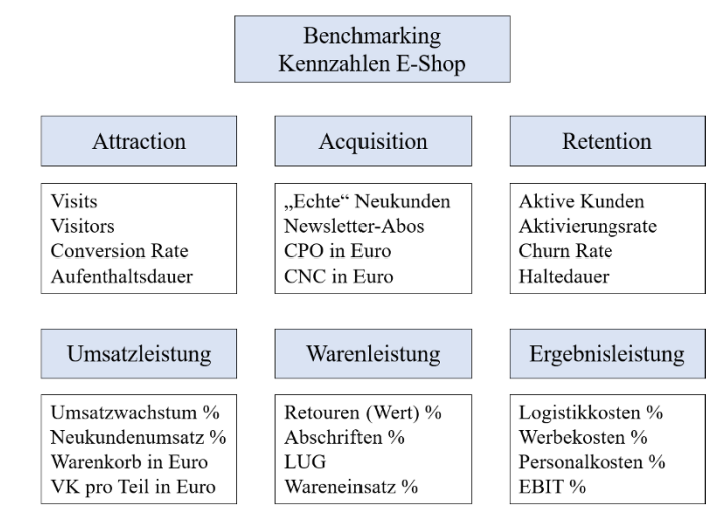
\includegraphics[width=8cm]{images/e-commerce_kennzahlen.png}
    \caption{Kennzahlen für Webshops in sechs Bereiche \cite{Gast2018}}
    \label{fig:kennzahlen}
\end{figure}

Die wichtigste Kennzahl für die Usability eines Webshops ist aber die Conversion Rate \cite{Gast2018}. Die Conversion Rate gibt an wie viele Besuche eines Webshops zu einem Erfolg führen (Erfolg: meistens Kauf eines Artikels). Berechnet wird die Conversion Rate durch die Anzahl der Erfolge * 1000 / Anzahl der Besuche. Das Ergebnis dieser Formel wird in Prozent angegeben. Dicht gepaart mit der Conversion Rate ist die Abbruchrate. Die Abbruchrate gibt an wie viel Prozent der Besucher keinen Kauf erfolgreich abschließen. Die Abbruchrate wird daher durch 1 - Conversion Rate errechnet \cite{Gast2018}.

Um die Conversion Rate zu verbessern müssen die Abbruchursachen identifiziert werden und den Benutzer einen simplen und verständlichen Weg bereitstellen einen Kauf abzuschließen.


\subsection{Vorgehen}
Für die Evaluation des Webshops wird eine Usability Inspection durchgeführt. Als konkrete Methode wird dabei die Heuristische Evaluation verwendet.

Der Grund für diese Entscheidung ist, dass die Usability Inspection bzw. Heuristische Evaluation eine sehr konstengünstige und effiziente Methode ist. Damit ist sie besonders attraktiv für E-Commerce Unternehmen mit begrenzten Resourcen bzw. Fachwissen über Usability. Die Methode ist für fast jeden Webshop umsetzbar, weswegen die Relevanz einer praktischen Evaluation dieser Methode gegeben ist. Die Heuristische Methode wird wie folgt durchgeführt:

\begin{enumerate}
  
  \item Zu Beginn der Evaluation wird aus den beschriebenen Heuristiken in Kapitel 1 ein Fragebogen (s. Anhang) erstellt.
  \item Anhand dieses Fragebogens werden von einem Experten Usability-Probleme identifiziert.
  \item Im Kapitel \ref{sec:Evaluation} werden dann die gefundenen Probleme beschrieben.
  \item Daraufhin wird jedes Problem bewertet. Für diese Bewertung wird die Scala aus dem Kapitel \ref{sec:heueva} verwendet. Dabei werden Usability-Probleme von einer Scala von null bis vier nach ihrer Schwere eingeordnet (0 = kein Problem, 4 = Usability-Katastrophe).
  \item Schlussendlich wird für beide Webshops das Gesamtergebniss dargestellt. Dabei wird die Anzahl der Probleme pro Heuristik in einem Balkendiagramm dargestellt. Zusätzlich wird die durschschnittliche Schwere der Probleme pro Heuristik berechnet und dargestellt. 
  Dadurch bekommt man einen guten Überblick wie gut die beiden Webshops bei der Heuristischen Evaluation abgeschnitten haben und welche Probleme besonders schwerwiegend sind.
\end{enumerate}
  

\subsection{Evaluation der Webshops}\label{sec:Evaluation}
In diesem Kapitel werden zwei Webshops mithilfe der Methode Usability Inspection evaluiert. Dabei wird das Vorgehen wie im vorherigen Kapitel beschrieben verwendet. Während der Evaluation wird vor allem auf die Usability-Probleme der Webshops eingegangen. Jedoch werden vereinzelnt besonders positive Aspekte herausgehoben. 

Für die Evaluation der zwei Webshops wurden die Webshops der Böttcher AG und Nike Inc. ausgewählt.


\subsubsection{Böttcher AG}
Die Böttcher AG ist ein deutscher Online-Händler für Büroartikel, die ihre Ware haupsächlich B2B vertreibt. Ihr Produktsortiment besteht aus knapp 200.000 Artikel und sie haben eine Kundenstamm von 7 Millionen Menschen \cite{böttcher}. Dabei fokusiert sich der Online-Händler auf Verbrauchsgegenstände im Büroalltag. Jedoch ist das Produktportfolio mittlerweile auf z.B. Arbeitskleidung und Werkzeuge erweitert. Ihrem Webshop erreicht man unter der URL \url{https://www.bueromarkt-ag.de/}. 


\subsubsection*{Ästhetisches und minimalistisches Design}
Der Webshop der Böttcher AG ist sehr überladen. Böttcher versucht auf der Startseite so viele Artikel wie möglich dem/der Nutzer*in anzubieten. Die eigentliche Intention einer Startseite ist jedoch dem/der Nutzer*in zu erlauben sich im Webshop zu navigieren. Besonders im B2B-Bereich haben die Nutzer*innen eine klare Vorstellung welche Produkte bestellt werden müssen. Es ist also fraglich wie sinnvoll das Werben von Produkten auf der Startseite ist. Das Problem ist, dass die Werbung viel Platz auf der Startseite verbraucht, die für wichtigere Funktionen genutzt werden kann. Dazu kommt das die verschiedenen Werbebereiche redundant sind. Es gibt zum Beispiel einen Bereich „Top-Empfehlungen für Sie“ und einen Bereich „Ausgewählte Artikel für Sie“. Diese Bereiche werden als unterschiedliche Funktionen verkauft, bedeuten aber dasselbe. (Schwere: 4)

Im Navigationsmenü werden ebenfalls verschiedene Werbe-/Angebotsbereiche verlinkt. Die eigentliche Navigation über die verschieden Produktkategorien befindet sich an letzter Stelle des Navigationsmenü. Die mit wichtigste Funktion der Startseite nimmt also eine sehr untergeordnete Rolle ein. Besser wäre es die Angebotsbereiche zu entfernen und das gesamte Navigationsmenü für die Navigation über die Kategorien zu nutzen. Durch den gewonnen Platz könnten die Kategorien noch feiner und untergliedert dargestellt werden. (Schwere: 2)

Auf der Startseite werden ebenfalls Kerndaten und Rezensionen des Webshops angezeigt. Auch diese Informationen sind für die Nutzer*innen an erster Stelle nicht relevant. Kunden im B2B-Bereich sind vorrangig Bestandskunden. Informationen über den Webshop sollten also auf einer getrennten Seite zu finden sein. Wenn Neukunden sich für diese Informationen interessieren, sollte die Startseite gut sichtbar auf diese Seite verweisen. (Schwere: 1)

Wählt man eine Kategorie aus werden erst weitere Empfehlungen und Filtermöglichkeiten angezeigt. Erst dann findet man eine Liste mit den Produkten der ausgewählten Kategorie. Bei kleineren Bildschirmen kann es sogar sein das die Produkte auf den ersten Blick gar nicht sichtbar sind. Man findet die Artikel nur durch das Scrollen nach unten. Die Filtermöglichkeiten sind außerdem nicht einklappbar. So kann es vorkommen das der Filterbereich die eigentlichen Artikel verdeckt, ohne dass der/die Nutzer*in diese Funktion nutzen möchte. (Schwere: 4)


\subsubsection*{Übereinstimmung von System und realer Welt}
Wählt man eine Kategorie aus kann man nur noch über eine „A-Z Leiste“ weiternavigieren. Wählt man einen Buchstaben auf dieser Leiste aus bekommt man alle Unterkategorien angezeigt, die mit diesem Buchstaben beginnen. Das Problem ist das Böttcher Kategorien anders benennen kann wie die Nutzer*innen erwarten. Sucht man z.B. unter dem Buchstaben K nach der Kategorie „Kugelschreiber“ findet man nichts. (Schwere: 3)

Die Sortierung der Unterkategorie nach dem Alphabet ist außerdem aus einem weiteren Grund unnatürlich. In einem physischen Geschäft werden die Produkte nicht nach dem Alphabet sortiert. In einem Supermarkt werden die Waren in Bereiche unterteilt. Innerhalb dieser Bereiche werden die Waren weiter unterteilt. Sucht man z.B. in einem Supermarkt nach einer Flasche Weißwein sucht man zuerst in der Getränkeabteilung. In dieser Abteilung sucht man den Bereich mit alkoholischen Getränken. Dort sucht man dann nach Weinen. Die natürliche Vorgehensweise ist das gesuchte Produkt in immer kleiner werden Kategorien zu suchen. (Schwere: 3)

Eine weitere Möglichkeit wie man zu dieser Leiste gelangt ist durch den Link „Artikel A-Z“ auf der Startseite. Wenn man weiß, wie die Navigationsfunktion hinter diesem Link funktioniert scheint diese Benennung sinnvoll. Weiß man aber nichts von dieser Funktion ist die Benennung verwirrend. Was sich hinter diesen Link nämlich befindet, ist eine Liste aller Artikel. Eine passendere Benennung des Links wäre also eher „alle Artikel“. (Schwere: 2)

Positiv ist das sich der Webshop in bestimmten Bereichen an bestimmte Normen hält. So ist es z.B. üblich, dass der Warenkorb in der rechten oberen Ecke durch ein Einkaufswagen-Icon erreicht werden kann. (Schwere: 0)


\subsubsection*{Erkennen vor Erinnern}
Anzumerken ist das die Ergebnisse dieser Heuristik für die Böttcher AG weniger relevant sind. Die Kunden im B2B-Bereich sind überwiegend Bestandskunden, die regelmäßig Produkte bestellen. Benutzt man den Shop regelmäßig erlernt man seine Funktionen. Diese Funktionen müssen also nicht jedes Mal neuerkannt werden.

Viele Funktionen des Webshops sind versteckt oder gehen unter. Der Link „Artikel A-Z“ ist z.B. sehr unauffällig über der Suchleisten platziert. Diese Funktion würde man eher im Navigationsmenü erwarten. Dort wäre die Funktion ihrer Bedeutung gerecht auffällig genug. (Schwere: 3)

Eine besonders gute Funktion ist die Einkaufsliste. In dieser Liste kann man Artikel über eine Sitzung hinweg speichern. Wenn regelmäßig Artikel nachbestellt werden kann man diese in der Einkaufsliste vermerken. Dadurch muss man sich nicht erinnern welches Produkt man das letzte Mal bestellt hat, sondern kann es aus der Einkaufsliste direkt in den Warenkorb verschieben. (Schwere: 0)

Eine weitere gute Funktion ist das Artikel über die Bestellnummer in den Warenkorb hinzugefügt werden können. Möchte man wieder bestimmte Artikel nachbestellen und hat diese nicht in der Einkaufsliste gespeichert, muss man nur die Bestellnummer der letzten Rechnung heraussuchen. (Schwere: 0)


\subsubsection*{Konsistenz und Standardisierung}
In dieser Heuristik schneidet der Webshop der Böttcher AG sehr schlecht ab. Oft passiert es dass ähnliche Aktionen zu unterschiedlichen Ergebnissen führen. Wählt man z.B. eine Kategorie aus, kann es sein das Empfehlungen oder Filtermöglichkeiten angezeigt werden. Wählt man eine andere Kategorie kann es sein das beides oder weder noch angezeigt wird. Diese Inkonsistenz sorgt für Verwirrung bei den Nutzer*innen, da sie das Gefühl bekommen in einem ganz anderen Bereich zu sein. (Schwere: 3)


\subsubsection*{Sichtbarkeit des Systemstatus}
In dieser Heuristik schneidet der Webshop positiv ab. Wenn ein/e Nutzer*in ein Produkt in den Warenkorb legt, wird durch eine grüne Erfolgsmeldung signalisiert das die Aktion erfolgreich war. Ebenfalls sehr positiv für die Sichtbarkeit des Systemstatus ist, dass der Gesamtpreis des Warenkorbs dem Nutzer immer angezeigt wird. Dadurch verliert der/die Nutzer*in nicht den Überblick wie viel er/sie gerade ausgibt. (Schwere: 0)

Dennoch gibt es kleinere Probleme. Ein Problem findet statt, wenn man im Warenkorb die Menge eines Produkts ändert. Das System setzt voraus, dass der/die Nutzer*in den Warenkorb manuelle aktualisieren muss, damit die Änderung durchgeführt wird. Der/Die Nutzer*in muss dabei auf einen unauffälligen Button drücken. Dieses manuelle Aktualisieren kann von dem/der Nutzer*in übersehen werden, was dann zu einer falschen Bestellung führen könnte. Der Zustand des Warenkorbs sollte sich demnach automatisch aktualisieren, wenn die Menge geändert wird. (Schwere: 2)


\subsubsection*{Benutzerkontrolle und Freiheit}
Der/Die Nutzer*in kann sich frei in dem Webshop bewegen. Teilweise müssen dabei die Funktionalitäten des Browser zur Unterstützung eingesetzt werden. Zum Beispiel gibt es kaum Möglichkeiten zurückzugehen. Diese Aktion passiert häufig und kann durch zusätzliche Buttons verbessert werden. Die Freiheiten der Nutzer*innen im Warenkorb sind standardmäßig. Man kann Artikel hinzufügen, entfernen und die Menge verändern. (Schwere: 1)

Eine wichtige Funktion die die Freiheit der Nutzer*innen erhöht sind Breadcrumbs. Diese Funktion stellt im Webshop der Böttcher AG die einzige Möglichkeit da, beliebige Stufen zurückzugehen. Gerade bei der unübersichtlichen Navigation im Webshop sind Breadcrumbs besonders wichtig. Leider ist diese Funktion ebenfalls sehr unauffällig gestaltet. Die Funktion geht trotz ihrer hohen Wichtigkeit auf der Webseite unter. (Schwere: 3)

Gegen das vertikale Scrollen wurde eine „Gehe nach oben“-Funktion eingeführt. Sobald man nach unten scrollt, erscheint ein Button, mit dem man wieder an den Anfang der Seite gelangt. Jedoch ist auch diese Funktion sehr versteckt. Der Text des Buttons hat eine hellgraue Farbe was auf dem weißen Hintergrund schwer erkennbar ist. (Schwere: 1)


\subsubsection*{Vermeiden von Fehlern}
Während der Evaluation konnte keine Mängel bezüglicher dieser Heuristik gefunden werden. (Schwere: 0)


\subsubsection*{Hilfe und Dokumentation}
Zur Hilfe wird den Nutzer*innen ein FAQ angeboten. Im Vergleich zu dem Webshop ist dieses sehr übersichtlich und minimal. Das FAQ beantwortet die wesentlichen Fragen. Es kann über den Footer der Webseite erreicht werden. Das ist eine übliche Positionierung, weswegen es keine Bedenken geben muss, dass man es nicht findet. (Schwere: 0)


\subsubsection*{Navigation und Suche}
Die Navigation ist recht kompliziert. Das kann daran liegen das Böttcher eine große Anzahl an verschiedene Produkte vertreibt. Kategorien sind meistens nicht logisch gruppiert, sondern stehen einzelnd. Das liegt daran das die Kategorie nach dem Alphabet sortiert sind. Deswegen kann es sein das ähnliche Kategorie sehr weit auseinander stehen. (Schwere: 3)

Die Navigationstruktur ist sehr breit angelegt. Jedoch muss man durch die große Anzahl an Artikel trotzdem sehr tief in den Navigationsbaum einschreiten. (Schwere: 1)

Durch die unauffällig Breadcrumbs-Funktion ist den Nutzer*innen nicht klar wo sie sich in der Navigationstruktur befinden. (Schwere: 2)

Positiv anzumerken ist die globale Suchfunktion. Auch wenn man diese nicht weiter einschränken kann, findet man durch die Suche häufiger die richtigen Artikel als mit der Navigation. (Schwere: 0)


\subsubsection*{Sprache}
Böttcher vertreibt seine Ware nur deutschlandweit, weswegen die Sprache weniger bedeutsam ist. (Schwere: 0)


\subsubsection{Nike Inc.}
Nike Inc. ist ein amerikanischer Sportartikelhersteller. Nike vertreibt seine Artikel hauptsächlich über einen eigenen Webshop. Im Vergleich zu Böttcher handelt es sich bei Nike um einen Lifestyle-Shop. Dementsprechend vertreiben sie ihre Artikel B2C. Lifestyle-Shops fokussieren sich auf Artikel, die im Zusammenhang mit einem aufstrebenden Lebensstil und Popkultur stehen. Nike erwirtschaftete durch ihren Webshop im Jahr 2021 einen Umsatz von 10 Milliarden US-Dollar \cite{Peters2022}. Den Webshop der Nike Inc. erreicht man unter der URL: \url{https://www.nike.com/de/}


\subsubsection*{Ästhetisches und minimalistisches Design}
Der Webshop von Nike ist sehr minimalistisch gehalten. Nike hat in diesem Aspekt auch einen gewissen Vorteil gegenüber Böttcher. Nike‘s Auswahl an verschiedenen Produkten ist wesentlich geringer als das Sortiment von Böttcher. Das vereinfacht z.B. die Navigation, da weniger Kategorien angeboten werden.

Insbesondere die Farbpalette ist sehr minimalistisch. Der Webshop ist grundsätzlich schwarz-weiß. Vereinzelt werden verschiedene Grautöne eingesetzt. Die einzigen farbigen Elemente im Webshop sind die Produkte selbst bzw. Werbungen für diese Produkte. Die Produktbilder sind im Vergleich zu Böttcher hochwertig produziert. Nike lenkt damit den Fokus der Nutzer*innen auf ihre Produkte. Der Webshop um die Produkte herum ist schlicht und minimalistisch gehalten. Die Funktionen sind auf die wichtigsten reduziert. Die Aufgabe des Webshops ist daher rein funktional. Durch das minimalistische Design wirkt der Webshop sehr übersichtlich und strukturiert.

Auch werden nur die wichtigsten Informationen angezeigt. Alle Informationen, die auf den ersten Blick nicht relevant sind, werden zu Beginn zugeklappt. Erst wenn ein Nutzer sich wirklich für eine Information interessiert, kann er diesen Bereich aufklappen. Zum Beispiel sind die Produktdetails oder Informationen zum Versand erst eingeklappt. (Schwere: 0)


\subsubsection*{Übereinstimmung von System und realer Welt}
Für diese Heuristik wurden im Webshop von Nike keine Mängel festgestellt. Funktionen und Bereiche werden konsistent gut benannt. Auch werden die Funktionen mit passenden Icons untermalt. (Schwere: 0)


\subsubsection*{Erkennen vor Erinnern}
Der Webshop von Nike verfügt über eine Funktion zum Speichern von Produkten über eine Sitzung hinweg. Diese Funktion heißt Favoriten. Gleich wie bei Böttcher sorgt diese Funktion, dass sich Kunden an Produkte nicht erinnern müssen. Durch diese Funktionen können Sie ihre Lieblingsprodukte auf einen Blick sehen. Die Funktion wird zusätzlich durch ein Herz-Icon verdeutlicht. Jedoch können Produkte nur über die Produktübersicht zu den Favoriten hinzugefügt werden. Über die Produktliste direkt ist es nicht möglich. Möchte ein Nutzer also die Produktliste überfliegen um Produkte, die im Gefallen in die Favoriten zu speichern muss dieser immer erst in die Produktübersicht. Nach dieser Aktion muss er/sie dann wieder zurück. Durch die Möglichkeit direkt von der Produktliste Produkte in den Favoriten zu speichern könnte der/die Nutzer*in diese Aktion effizienter ausführen. (Schwere: 0)

Eine Funktion, die etwas unnatürlich ist, ist das Ein- und Ausklappen der Filterfunktion. Die Filterfunktion befindet sich auf der linken Seite des Webshops. Das Icon, um die Filterfunktion ein- und auszuklappen, befindet sich jedoch auf der rechten Seite. Diese Platzierung ist sehr unnatürlich für die Nutzer*innen. Besser wäre, dass das Filter-Icon ebenfalls auf der linken Seite platziert wäre, damit klarer wird dass das Icon mit der Filterfunktion korreliert. (Schwere: 1)


\subsubsection*{Konsistenz und Standardisierung}
Der Webshop hat eine hervorragende Konsistenz. Unabhängig von der Kategorie der Produkte sehen Produktliste und Produktübersicht identisch aus. Dadurch sind die Nutzer weniger verwirrt und müssen sich nicht verschiedene Vorgehensweisen aneignen. (Schwere: 0)


\subsubsection*{Sichtbarkeit des Systemstatus}
Befindet man sich in der Produktliste werden, wenn man weiter nach unten scrollt weitere Produkte angezeigt. Der Nike Shop verzichtet also auf eine Pagination-Funktion. Das Laden neuer Produkte ist eine asynchrone Aktion, die von der Netzwerkverbindung zum dahinter liegenden Anwendungsserver abhängt. Aus diesem Grund kann es sein, dass der Nutzer auf der Clientseite schon das Ende der Seite erreicht, der Webshop aber noch nicht alle Produkte geladen hat. Dieser Systemstatus wird den Nutzer*innen passend mit einem Ladebalken signalisiert. (Schwere: 0)

Parallel zum Webshop von Böttcher wird den Nutzer*innen bestätigt, wenn sie erfolgreich ein Produkt in den Warenkorb oder zu den Favoriten hinzugefügt haben. Bei Nike wird ein kleines Menü angezeigt, welches das Produkt anzeigt und Links zu den Favoriten bzw. zum Warenkorb bereitstellt. Dieses Menü wird weiter hervorgehoben, indem der Webshop im Hintergrund dunkler wird. Möchte man normal fortfahren muss man das Menü manuell schließen. Diese Aktion kann sehr repetitiv werden wenn man oft Produkte zu dem Warenkorb oder zu den Favoriten hinzufügt. Auf der anderen Seite geht Nike damit sicher, dass der/die Nutzer*in erkannt hat das die Aktion erfolgreich war. (Schwere: 0)

Negativ bei Nike ist, dass der Webshop nicht den aktuellen Gesamtpreis des Warenkorbs immer anzeigt. Um die Gesamtsumme zu sehen, muss man den Warenkorb öffnen. (Schwere: 1)


\subsubsection*{Benutzerkontrolle und Freiheit}
Parallel zum Webshop von Böttcher gib es wenige Zurück-Buttons. Auch hier muss man für diese Funktion die Browserfunktionalitäten zur Unterstützung benutzen Die einzige Alternative ist ebenfalls die Breadcrumb-Funktion. Diese Funktion ist aber ähnlich zu Böttcher unauffällig platziert. (Schwere: 3)

Der Webshop von Nike verzichtet auf eine Pagination-Funktion. Anstelle davon werden neue Produkte geladen, sobald man weiter nach unten scrollt. Aus Nutzersicht fühlt diese Funktion sich natürlicher an, da man einfach die Scroll-Aktion weiterführen kann. Jedoch birgt diese Funktion auch einige Gefahren.

\begin{enumerate}
  \item Wenn ein/e Nutzer*in weiß das ein Produkt weiter hinten in der Liste auftaucht muss er/sie ganz nach unten scrollen und kann nicht Seiten überspringen.
  \item Möchte man zum Footer gelangen muss man ebenfalls bis zum Ende scrollen, weil sonst immer weitere Inhalte geladen werden. (Schwere: 1)
\end{enumerate}

Potenzial wurde beim Bestätigungs-Menü , das auftaucht wenn man Produkte in den Warenkorb oder zu den Favoriten hinzufügt, verschwendet. Durch einen extra Button könnte man den Nutzer*innen erlauben die getätigte Aktion rückgängig zu machen. Diese Funktion würde den Nutzern noch mehr Freiheit gewähren. Hat man beispielsweise fälschlicherweise ein Produkt in den Warenkorb getan, muss man aktuell erst in den Warenkorb um dieses wieder zu entfernen. (Schwere: 1)


\subsubsection*{Vermeiden von Fehlern}
Während der Evaluation konnte keine Mängel bezüglicher dieser Heuristik gefunden werden. (Schwere: 0)


\subsubsection*{Hilfe und Dokumentation}
Die Hilfe kann im Footer gefunden werden. Das ist ein üblicher Platz, wo man eine Hilfe finden würde. Die Hilfe an sich besteht aus zwei Teilen. Teil 1 ist eine Suchfunktion, mit der man nach Fragen und deren antworten suchen kann. Diese Funktion ist also ein sehr ausführliches FAQ. Teil 2 sind verschieden Kontaktinformationen. So kann man für verschiedene Themen verschieden Hotlines anrufen. Außerdem kann man per Chatfunktion mit Support-Mitarbeitern chatten. Zudem zeigt der Webshop den nächsten physischen Shop zum eigenen Standort an, sodass dort vor Ort mit einem Mitarbeiter gesprochen werden kann. (Schwere: 0)


\subsubsection*{Navigation und Suchfunktion}
Die Navigation ist sehr gut. Die Navigation ist simpel und logisch gehalten. Die verschiedenen Kategorien werden bestimmten logischen Bereichen zugeordnet, weswegen man schnell zu den gewünschten Produkten findet. (Schwere: 0)

Die Navigation ist ebenfalls sehr breit angelegt. Durch die geringere Anzahl an Produkten im Vergleich zu Böttcher schafft Nike, dass der/die Nutzer*in nicht tief in den Navigationsbaum eintreten muss. Aufgrund der geringen Tiefe ist es für den/die Nutzer*in auch einfacher zu erkennen wo er/sie sich in der Navigationstruktur befindet. Deswegen ist in diesem Fall die unauffällig Breadcrumb-Funktion zu vernachlässigen. (Schwere: 0)

Besonders hervorzuheben ist die Suchfunktion des Webshops. Dem Nutzer werden passende Vorschläge für den Suchbegriff angegeben. Zusätzlich werden gleich Produkte mit Produktbilder, Name und Preis angezeigt. Dadurch ist die Sucher sehr übersichtlicht. (Schwere: 0)


\subsubsection*{Sprache}
Nike passt beim Starten des Webshops die Sprache automatisch zur Staatssprache am aktuellen Standort an. Befindet man sich in Deutschland wird man automatisch zu deutschen Variante des Webshops gebracht. 

Manuell die Sprache zu ändern ist möglich, jedoch ist diese Funktion versteckt. So befindet sich ganzen unten im Footer ein Link mit dem man manuelle seinen Standort ändern kann. Diese Funktion ist erstens schwer zu finden und zweitens macht die Funktion nicht klar, dass wenn man den Standort wechselt dass dann die Sprache auch wechselt. 

Die Funktion die Sprache ändern zu können sollte deutlicher platziert sein. Wenn ein/e Benutzer*in nicht die Sprache ihres aktuellen Standortes spricht wird er/sie Schwierigkeiten haben diese zu wechseln. (Schwere: 2)


\subsection*{Ergebnis}
In diesem Kapitel werden die Ergebnisse der Evaluation zusammengefasst. Dabei werden jeweils die drei größten Usability-Probleme der beiden Webshops noch einmal dargestellt. Daraufhin wird die Anzahl der Usability-Probleme pro Schwere der beiden Webshops gegenübergestellt. Anmerkungen aus dem Kapitel \ref{sec:Evaluation} die mit der Schwere 0 (kein Usability-Problem) gekennzeichnet sind, werden dabei weggelassen. Schlussendlich wird die durchschnittliche Schwere der Usability-Probleme pro Heuristik gegenübergestellt. Bei der Berechnung des Durschnitts, werden ebenfalls Anmerkungen mit der Schwere 0 weggelassen, da diese das Ergebnis verfälschen würden. 

Die drei größten Usability-Probleme des Webshops der Böttcher AG:
\begin{enumerate}
  \item Webshop ist mit Information und Funktionen überladen (redundaten Funktionen, Werbung, ...)
  \item Wichtige Informationen wie z.B. die Produktliste sind außerhalb der direkten Sichtfläche der Nutzer*innen, da z.B. Filterfunktionen ihnen den Platz wegnehmen.
  \item Keine Konsistenz.
\end{enumerate}


Die drei größten Usability-Probleme des Webshops der Nike Inc.:
\begin{enumerate}
  \item Unauffällige Breadcrumbs
  \item Manuelle Sprachänderung ist nicht intuitiv, da Standort geändert werden muss.
  \item Aktueller Gesamtpreis des Warenkorbs wird nur im Warenkorb selbst angezeigt.
\end{enumerate}

Im folgenden Balkendiagramm werden die Anzahl der Fehler, unterteilt in Schwere pro Heuristik, angezeigt. Die Werte der Böttcher AG befinden sich jeweils Links vom X-Wert und die Werte von Nike befinden sich rechts vom X-Wert. Außerdem sind die Werte der Böttcher AG heller als die von Nike. Man kann erkennen, dass für den Webshop von Böttcher wesentlich mehr Probleme identifiziert wurden.

\pgfplotsset{width=14cm,compat=1.8}

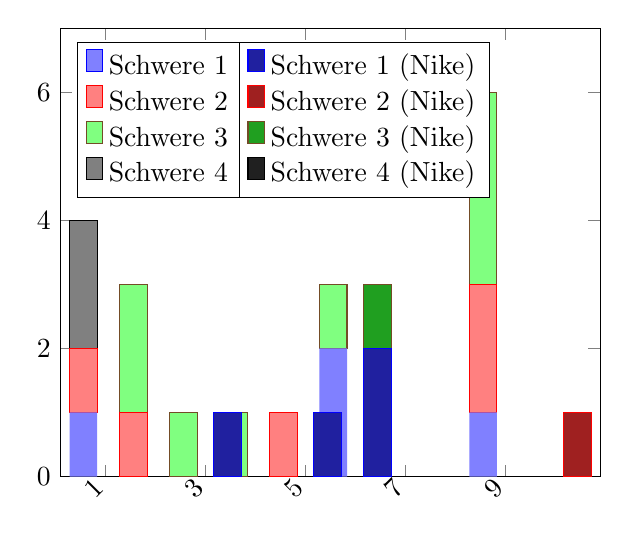
\begin{tikzpicture}[ every axis/.style={symbolic x coords={1,2,3,4,5,6,7,8,9,10}}]

\begin{axis}[ybar stacked,ymin=0,ymax=7, bar shift=-8pt,  x tick label 
style={rotate=45,anchor=east}, legend style={at={(0.03,0.97)}, anchor=north west, legend cell align=left, align=left, draw=black}]  
\addplot+[fill=blue!50, draw=none] coordinates {(1,1) (2,0) (3,0) (4,0) (5,0) (6,2) (7,0) (8,0) (9,1) (10,0)};
\addlegendentry{Schwere 1 (Böttcher)}
\addplot+[fill=red!50] coordinates {(1,1) (2,1) (3,0) (4,0) (5,1) (6,0) (7,0) (8,0) (9,2) (10,0)};
\addlegendentry{Schwere 2 (Böttcher)}
\addplot+[fill=green!50] coordinates {(1,0) (2,2) (3,1) (4,1) (5,0) (6,1) (7,0) (8,0) (9,3) (10,0)};
\addlegendentry{Schwere 3 (Böttcher)}
\addplot+[fill=black!50] coordinates {(1,2) (2,0) (3,0) (4,0) (5,0) (6,0) (7,0) (8,0) (9,0) (10,0)};
\addlegendentry{Schwere 4 (Böttcher)}
\end{axis}

\begin{axis}[ybar stacked,ymin=0,ymax=7, bar shift=8pt,  x tick label 
style={rotate=45,anchor=east}, hide axis, legend style={at={(0.33,0.97)}, anchor=north west, legend cell align=left, align=left, draw=black}] 
\addplot+[fill=blue!50!darkgray] coordinates {(1,0) (2,0) (3,1) (4,0) (5,1) (6,2) (7,0) (8,0) (9,0) (10,0)};
\addlegendentry{Schwere 1 (Nike)}
\addplot+[fill=red!50!darkgray] coordinates {(1,0) (2,0) (3,0) (4,0) (5,0) (6,0) (7,0) (8,0) (9,0) (10,1)};
\addlegendentry{Schwere 2 (Nike)}
\addplot+[fill=green!50!darkgray] coordinates {(1,0) (2,0) (3,0) (4,0) (5,0) (6,1) (7,0) (8,0) (9,0) (10,0)};
\addlegendentry{Schwere 3 (Nike)}
\addplot+[fill=black!50!darkgray] coordinates {(1,0) (2,0) (3,0) (4,0) (5,0) (6,0) (7,0) (8,0) (9,0) (10,0)};
\addlegendentry{Schwere 4 (Nike)}
\end{axis}
%\begin{axis}[ybar stacked,ymin=0,ymax=11,symbolic x coords=
%{1,2,3,4,5}]  
%\addplot+[fill=blue!50!gray] coordinates
%{(1,1.5) (2,1.5) (3,3.5) (4,2.5) 
%(5,1)};
%\end{axis}

%\begin{axis}[ybar stacked,bar shift=-8pt,ymin=0,ymax=11,symbolic x coords=
%{White Other,African Caribbean and White,African,D,E}]  
%\addplot+[fill=blue!50!gray] coordinates
%{(White Other,1.5) (African Caribbean and White,1.5) (African,3.5) (D,2.5) 
%(E,1)};
%\end{axis}
\end{tikzpicture}

Im folgenden Diagramm wird die durchschnittliche Schwere der Probleme pro Heuristik angezeigt. Dabei werden die Werte von Böttcher blau dargestellt. Die Werte von Nike werden orange dargestellt. Man kann erkennen das die Probleme des Webshops von Böttcher durchschnittlich schwerer ausfallen wie die von Nike. Außerdem erkennt man das bei Böttcher vorallem Probleme bei den Heuristiken 1 bis 6 sowie 9 bestehen. Nikes Probleme liegen bei der Heuristik 6 und 10. 

\begin{tikzpicture}
\tkzKiviatDiagram[scale=.5,label distance=.5cm,
        radial  = 4,
        gap     = 1,  
        lattice = 4]{1,2,3,4,5,6,7,8,9,10}
\tkzKiviatLine[thick,color=blue,mark=ball,mark size=4pt,
               fill=blue!20,opacity=.5](2.75,2.66,4,4,3,2.66,1,1,3,1)  
\tkzKiviatLine[thick,color=orange,mark=ball,mark size=4pt, ball color=orange,
               fill=orange!30,opacity=.5](1,1,2,1,2,2.66,1,1,1,3)  
\tkzKiviatGrad[prefix=,unity=1,suffix=](1)  
\end{tikzpicture}


\subsection{Vergleich der Anwendbarkeit}
Die Methode der Heuristischen Evaluation ist sehr konstengünstig. Aus diesem Grund kann man sie fast immer zur Verbesserung der Usability einsetzen. Vor allem kann man die Methode schon frühzeitig während der Entwicklung des Webshops einsetzten. Ein/e Entwickler*in/Designer*in hat einen geringen Mehraufwand während der Entwicklung die Heuristiken zu beachten. 

Mit der Methode schafft man es große Usability-Probleme oder Katastrophen zu verhindern. Je weniger schwer die Probleme jedoch werden, desto höher ist die Gefahr Scheinprobleme zu identifizieren. Möchte man also im Detail auch kleinere Usability-Probleme identifizieren, muss eine qualitativere Methode in Zusammenarbeit mit den Kund*innen gewählt werden.

Ein Thema bei dem die Heuristische Evaluation kein gutes Ergebnis erzielen konnte ist die Navigation. Es ist schwer für die Navigation eine Heuristik zu definieren. Die Navigation hängt stark von der Intuition der Nutzer*innen eines Webshops ab. Deswegen ist die Formulierung einer allgemeingültigen Heuristik für die Navigation schwierig. Für die Verbesserung der Navigation müssen also Methoden verwendet werden, die die Nutzer*innen mit einbeziehen (z.B. Beobachtung oder Befragung). 

Gute Ergebnisse erzielte die Methode beim Thema Konsistenz und minimalistisches Design. Bei diesem Heuristiken geht es um die klare und deutliche Darstellung von Informationen. Für diese Aspekte kann man sehr gut allgemeingültige Regeln definieren. 

Die Heuristik \glqq Erkennen vor Errinern\grqq{} scheint bei dem Webshop von Böttcher und ähnlichen Webshops weniger relevant. B2B-Geschäfte haben oft Bestandskunden die immer wieder bei dem Webshop Ware nachbestellen. Aus diesem Grund können die Nutzer*innen die Funktion des Webshops erlernen. Deswegen sind sie weniger wahrscheinlich darauf angewiesen Funktionen zu erkennen.

Bei Lifestyle-Shops wie Nike scheint die Heuristik \glqq minimalistisches und ästhetisches Design\grqq{} besonders wichtig zu sein. Lifestyleshops sind ausgelegt, dass die Nutzer*innen gerne durch den Webshop stöbern. Durch ein ästhetisches Design und hochwertige Produktbilder bleiben die Nutzer*innen gerne im Shop um diese schönen Dinge zu betrachten.

Schlussendlich kann man sagen das die Methode der Heuristischen Evaluation für den durchschnittlichen Webshop eine gute Methode ist. Für einen besseren Erfolg dieser Methode muss mit dem Heuristikbogen weiter experimentiert werden, um diese noch genauer auf die Usability von Webshops zu zuschneiden. Um den Erfolg dieser Methode messbar zu machen müssen die identifizierten Usability-Probleme umgesetzt werden und einen Vorher-Nachher-Vergleich durchführen.

\clearpage



\section{Fazit}
Im folgenden Kapitel werden die Ergebnisse der Seminararbeit präsentiert und kritisch beleuchtet. Außerdem wird ein Ausblick gegeben.


\subsection*{Ergebnisse}
Es wurden verschiedene Heuristiken der Usability recherchiert und gegenübergestellt. Die Heuristiken wurden in einer Tabelle (\ref{table:tab1}) dargestellt. Daraufhin wurden die konkreten Vorgehensweisen Usability Inspection, Menschzentrierte Gestaltung und der Usability Engineering Lifecycle zur Sicherstellung der Heuristiken erarbeitet und verglichen. Auf Grundlage der Heuristiken und der Vorgehensweisen wurden nun zwei Webshops evaluiert. Hierfür wurden die Heuristische Evaluation verwendet, sowie die erarbeiteten Heuristiken der Tabelle.


\subsection*{Kritische Würdigung}
Die Ziele der Arbeit konnten erreicht werden. Zusätzlich zu den erarbeiteten Heuristiken könnten weitere Heuristiken anderer Quellen betrachtet werden. Die Evaluation könnte weiter verbessert werden, indem man die verwendeten Heuristiken und den Fragebogen überarbeitet. Bei der Überarbeitung sollten die Heuristiken noch spezifischer für Webshops angepasst werden. Außerdem konnten der Erfolg der Evaluation nicht messbar überprüft werden. Für eine messbare Überprüfung müssten die Probleme der Webshops verbessert werden und dann ein Vorher-Nachher-Vergleich durchgeführt werden.


\subsection*{Ausblick}
Da sich Normen und Standards zu Gestaltung und Usability häufig ändern, sollten die Heuristiken in Zukunft ständig überprüft und bei Bedarf aktualisiert und überarbeitet werden. Dies gilt auch für die Vorgehensweisen zur Evaluierung. 

\newpage
\printbibliography

\newpage
\begin{appendices}
\section{Heuristikbogen}\label{sec:Heuristikbogen}
\begin{enumerate}
  \item \textbf{Minimalistisches Design}
  \begin{itemize}
    \item Werden zu jedem Zeitpunkt nur die nötigsten Informationen angezeigt?
    \item Werden weitere Informationen ausgelagert (z.B. in Hilfsdialoge)
    \item Sind gruppierte Elemente als solche gekennzeichnet?
    \item Folgt die Platzierung der Elemente dem natürlichen Lesefluss?
    \item Werden wenige schlichte Farben verwendet?
    \item Kann man die Benutzeroberfläche auch ohne Farbe nutzen?
    \item Werden keine Farben zur Informationsbereitstellung verwendet?
    \item Werden Nutzer*innen keine unnötigen Optionen angeboten?
    \item Werden die Informationen möglichst auf einen Singel Screen dargestellt?
  \end{itemize}
  \item \textbf{Übereinstimmung von System und realer Welt}
  \begin{itemize}
    \item Entspricht die Terminologie des Webshops der Sprache der Nutzer*innen?
    \item Werden Icons zur Symbolisierung von Informationen verwendet?
    \item Werden merhdeutige Worte vermieden?
    \item Werden alle Interaktionen aus der Sicht der Nutzer*innen formuliert?
    \item Kann ein Nutzer Aliase definieren?
  \end{itemize}
  \item \textbf{Erkennen vor Errinern}
  \begin{itemize}
    \item Unterstützt der Webshop den Nutzer beim Errinern von Informationen?
    \item Basiert der Webshop aus einer kleinen Menge an Regeln?
  \end{itemize}
  \item \textbf{Konsistenz und Standardisierung}
  \begin{itemize}
    \item Führen ähnliche Aktionen zu denselben oder ähnlichen Ergebnissen?
    \item Findet man die gleichen Informationen immer an der selben Stelle?
    \item Befinden sich Informationen, die sich auf einander beziehen in der gleichen Reihenfolge?
  \end{itemize}
  \item \textbf{Sichtbarkeit des Systemstatus}
  \begin{itemize}
    \item Wird der/die Nutzer*in informiert, wie das System einen Input interpretiert?
    \item Wird der/die Nutzer*in informiert, was das System mit dem Input macht?
    \item Werden Aktionen mit langer Antwortzeit gekennzeichnet?
    \item Werden bei Systemfehlern informative Fehlermeldungen angezeigt?
  \end{itemize}
  \item \textbf{Benutzerkontrolle und Freiheit}
  \begin{itemize}
    \item Kann man alle Dialoge verlassen?
    \item Kann man Aktionen rückgängig machen ?
    \item Kann man bei Wartezeiten den Prozess abbrechen?
  \end{itemize}
  \item \textbf{Vermeiden von Fehler}
  \begin{itemize}
    \item Fängt das System Fehler ab, bevor eine Fehlermeldung kommt?
    \item Sind Fehlermeldungen klar und verständlich?
    \item Sind Fehlermeldungen präzise formuliert?
    \item Hilft die Fehlermeldung dem/der Nutzer*in das Problem zu lösen?
    \item 
  \end{itemize}
  \item \textbf{Hilfe und Dokumentation}
  \begin{itemize}
    \item Ist die Dokumentation vollständig und verständlich?
    \item Ist die Dokumentation zugänglich?
    \item Ist die Dokumentation auf dem aktuellsten Stand?
    \item Stellt die Dokumentation Kontaktinformationen bereit?
  \end{itemize}
  \item \textbf{Navigation und Suche}
  \begin{itemize}
    \item Macht die Navigation deutlich wo sich der/die Benutzer*in in der Navigationsstruktur befindet?
    \item Werden verschiedene Navigationsstrategien angeboten?
    \item Ist die Navigation einfach gehalten?
    \item Sind Verknüpfungen logisch gruppiert und sinnvoll benannt?
    \item Ist die Navigationsstruktur breit angelegt?
    \item Ist die Navigationsstruktur konsistent?
    \item Bietet der Webshop eine Suchfunktion an?
    \item Ist die Suche global zugänglich?
    \item Sind die Suchergebnisse sinnvoll angeordnet?
    \item Sind die Suchergebnisse ausreichend gut beschrieben?
    \item Kann die Suche weiter eingeschränkt werden?
  \end{itemize}
  \item \textbf{Sprache}
  \begin{itemize}
    \item Werden verschiedene Sprachen unterstützt?
    \item Ist die Sprache global einstellbar?
  \end{itemize}
\end{enumerate}
\end{appendices}
\end{document}
